\documentclass[twoside]{book}

% Packages required by doxygen
\usepackage{fixltx2e}
\usepackage{calc}
\usepackage{doxygen}
\usepackage[export]{adjustbox} % also loads graphicx
\usepackage{graphicx}
\usepackage[utf8]{inputenc}
\usepackage{makeidx}
\usepackage{multicol}
\usepackage{multirow}
\PassOptionsToPackage{warn}{textcomp}
\usepackage{textcomp}
\usepackage[nointegrals]{wasysym}
\usepackage[table]{xcolor}

% Font selection
\usepackage[T1]{fontenc}
\usepackage[scaled=.90]{helvet}
\usepackage{courier}
\usepackage{amssymb}
\usepackage{sectsty}
\renewcommand{\familydefault}{\sfdefault}
\allsectionsfont{%
  \fontseries{bc}\selectfont%
  \color{darkgray}%
}
\renewcommand{\DoxyLabelFont}{%
  \fontseries{bc}\selectfont%
  \color{darkgray}%
}
\newcommand{\+}{\discretionary{\mbox{\scriptsize$\hookleftarrow$}}{}{}}

% Page & text layout
\usepackage{geometry}
\geometry{%
  a4paper,%
  top=2.5cm,%
  bottom=2.5cm,%
  left=2.5cm,%
  right=2.5cm%
}
\tolerance=750
\hfuzz=15pt
\hbadness=750
\setlength{\emergencystretch}{15pt}
\setlength{\parindent}{0cm}
\setlength{\parskip}{0.2cm}
\makeatletter
\renewcommand{\paragraph}{%
  \@startsection{paragraph}{4}{0ex}{-1.0ex}{1.0ex}{%
    \normalfont\normalsize\bfseries\SS@parafont%
  }%
}
\renewcommand{\subparagraph}{%
  \@startsection{subparagraph}{5}{0ex}{-1.0ex}{1.0ex}{%
    \normalfont\normalsize\bfseries\SS@subparafont%
  }%
}
\makeatother

% Headers & footers
\usepackage{fancyhdr}
\pagestyle{fancyplain}
\fancyhead[LE]{\fancyplain{}{\bfseries\thepage}}
\fancyhead[CE]{\fancyplain{}{}}
\fancyhead[RE]{\fancyplain{}{\bfseries\leftmark}}
\fancyhead[LO]{\fancyplain{}{\bfseries\rightmark}}
\fancyhead[CO]{\fancyplain{}{}}
\fancyhead[RO]{\fancyplain{}{\bfseries\thepage}}
\fancyfoot[LE]{\fancyplain{}{}}
\fancyfoot[CE]{\fancyplain{}{}}
\fancyfoot[RE]{\fancyplain{}{\bfseries\scriptsize Generated on Sun Oct 25 2015 10\+:53\+:20 for os\+\_\+4 by Doxygen }}
\fancyfoot[LO]{\fancyplain{}{\bfseries\scriptsize Generated on Sun Oct 25 2015 10\+:53\+:20 for os\+\_\+4 by Doxygen }}
\fancyfoot[CO]{\fancyplain{}{}}
\fancyfoot[RO]{\fancyplain{}{}}
\renewcommand{\footrulewidth}{0.4pt}
\renewcommand{\chaptermark}[1]{%
  \markboth{#1}{}%
}
\renewcommand{\sectionmark}[1]{%
  \markright{\thesection\ #1}%
}

% Indices & bibliography
\usepackage{natbib}
\usepackage[titles]{tocloft}
\setcounter{tocdepth}{3}
\setcounter{secnumdepth}{5}
\makeindex

% Hyperlinks (required, but should be loaded last)
\usepackage{ifpdf}
\ifpdf
  \usepackage[pdftex,pagebackref=true]{hyperref}
\else
  \usepackage[ps2pdf,pagebackref=true]{hyperref}
\fi
\hypersetup{%
  colorlinks=true,%
  linkcolor=blue,%
  citecolor=blue,%
  unicode%
}

% Custom commands
\newcommand{\clearemptydoublepage}{%
  \newpage{\pagestyle{empty}\cleardoublepage}%
}


%===== C O N T E N T S =====

\begin{document}

% Titlepage & ToC
\hypersetup{pageanchor=false,
             bookmarks=true,
             bookmarksnumbered=true,
             pdfencoding=unicode
            }
\pagenumbering{roman}
\begin{titlepage}
\vspace*{7cm}
\begin{center}%
{\Large os\+\_\+4 }\\
\vspace*{1cm}
{\large Generated by Doxygen 1.8.9.1}\\
\vspace*{0.5cm}
{\small Sun Oct 25 2015 10:53:20}\\
\end{center}
\end{titlepage}
\clearemptydoublepage
\tableofcontents
\clearemptydoublepage
\pagenumbering{arabic}
\hypersetup{pageanchor=true}

%--- Begin generated contents ---
\chapter{File Index}
\section{File List}
Here is a list of all files with brief descriptions\+:\begin{DoxyCompactList}
\item\contentsline{section}{/home/beebop/src/os\+\_\+4/src/\hyperlink{kernel_8c}{kernel.\+c} }{\pageref{kernel_8c}}{}
\item\contentsline{section}{/home/beebop/src/os\+\_\+4/src/\hyperlink{port_8c}{port.\+c} }{\pageref{port_8c}}{}
\item\contentsline{section}{/home/beebop/src/os\+\_\+4/src/\hyperlink{port_8h}{port.\+h} }{\pageref{port_8h}}{}
\item\contentsline{section}{/home/beebop/src/os\+\_\+4/src/\hyperlink{version_8h}{version.\+h} }{\pageref{version_8h}}{}
\item\contentsline{section}{/home/beebop/src/os\+\_\+4/src/\hyperlink{vga_8c}{vga.\+c} }{\pageref{vga_8c}}{}
\item\contentsline{section}{/home/beebop/src/os\+\_\+4/src/\hyperlink{vga_8h}{vga.\+h} }{\pageref{vga_8h}}{}
\item\contentsline{section}{/home/beebop/src/os\+\_\+4/src/init/\hyperlink{init_8c}{init.\+c} }{\pageref{init_8c}}{}
\end{DoxyCompactList}

\chapter{File Documentation}
\hypertarget{init_8c}{}\section{/home/beebop/src/os\+\_\+4/src/init/init.c File Reference}
\label{init_8c}\index{/home/beebop/src/os\+\_\+4/src/init/init.\+c@{/home/beebop/src/os\+\_\+4/src/init/init.\+c}}

\hypertarget{kernel_8c}{}\section{/home/beebop/src/os\+\_\+4/src/kernel.c File Reference}
\label{kernel_8c}\index{/home/beebop/src/os\+\_\+4/src/kernel.\+c@{/home/beebop/src/os\+\_\+4/src/kernel.\+c}}
{\ttfamily \#include \char`\"{}vga.\+h\char`\"{}}\\*
Include dependency graph for kernel.\+c\+:
\nopagebreak
\begin{figure}[H]
\begin{center}
\leavevmode
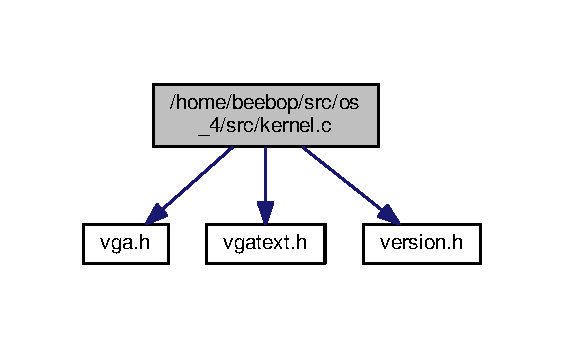
\includegraphics[width=188pt]{kernel_8c__incl}
\end{center}
\end{figure}
\subsection*{Functions}
\begin{DoxyCompactItemize}
\item 
void \hyperlink{kernel_8c_ada8402e0c504af8cafef5cc76c076003}{kernel\+\_\+main} ()
\end{DoxyCompactItemize}
\subsection*{Variables}
\begin{DoxyCompactItemize}
\item 
int \hyperlink{kernel_8c_a76453a26fc446453c0ace6a7faf3063e}{col} \mbox{[}$\,$\mbox{]}
\end{DoxyCompactItemize}


\subsection{Function Documentation}
\hypertarget{kernel_8c_ada8402e0c504af8cafef5cc76c076003}{}\index{kernel.\+c@{kernel.\+c}!kernel\+\_\+main@{kernel\+\_\+main}}
\index{kernel\+\_\+main@{kernel\+\_\+main}!kernel.\+c@{kernel.\+c}}
\subsubsection[{kernel\+\_\+main}]{\setlength{\rightskip}{0pt plus 5cm}void kernel\+\_\+main (
\begin{DoxyParamCaption}
{}
\end{DoxyParamCaption}
)}\label{kernel_8c_ada8402e0c504af8cafef5cc76c076003}


\subsection{Variable Documentation}
\hypertarget{kernel_8c_a76453a26fc446453c0ace6a7faf3063e}{}\index{kernel.\+c@{kernel.\+c}!col@{col}}
\index{col@{col}!kernel.\+c@{kernel.\+c}}
\subsubsection[{col}]{\setlength{\rightskip}{0pt plus 5cm}int col\mbox{[}$\,$\mbox{]}}\label{kernel_8c_a76453a26fc446453c0ace6a7faf3063e}
{\bfseries Initial value\+:}
\begin{DoxyCode}
= \{
  0x1, 0x9, 0x3, 0xb,
  0x2, 0xa, 0x6, 0xe,
  0x4, 0xc, 0x5, 0xd,
  0x8, 0x7, 0xf, 0x0
\}
\end{DoxyCode}

\hypertarget{port_8c}{}\section{/home/beebop/src/os\+\_\+4/src/port.c File Reference}
\label{port_8c}\index{/home/beebop/src/os\+\_\+4/src/port.\+c@{/home/beebop/src/os\+\_\+4/src/port.\+c}}
{\ttfamily \#include \char`\"{}port.\+h\char`\"{}}\\*
Include dependency graph for port.\+c\+:\nopagebreak
\begin{figure}[H]
\begin{center}
\leavevmode
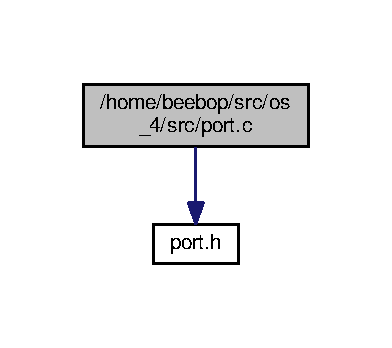
\includegraphics[width=188pt]{port_8c__incl}
\end{center}
\end{figure}
\subsection*{Functions}
\begin{DoxyCompactItemize}
\item 
void \hyperlink{port_8c_a758def1b1168d2562f6e5030e343240a}{outb} (unsigned short port, unsigned char val)
\item 
unsigned char \hyperlink{port_8c_a8e267bc99eb4e47d1390903b8ea0e522}{inb} (unsigned short port)
\item 
void \hyperlink{port_8c_ab33f4442a8212007469ac760323d9d2a}{outw} (unsigned short port, unsigned short val)
\item 
unsigned short \hyperlink{port_8c_a6d87b47abf48abc5f8dbc9788b3e26a3}{inw} (unsigned short port)
\end{DoxyCompactItemize}


\subsection{Function Documentation}
\hypertarget{port_8c_a8e267bc99eb4e47d1390903b8ea0e522}{}\index{port.\+c@{port.\+c}!inb@{inb}}
\index{inb@{inb}!port.\+c@{port.\+c}}
\subsubsection[{inb}]{\setlength{\rightskip}{0pt plus 5cm}unsigned char inb (
\begin{DoxyParamCaption}
\item[{unsigned short}]{port}
\end{DoxyParamCaption}
)}\label{port_8c_a8e267bc99eb4e47d1390903b8ea0e522}
Reads one byte from a port. 
\begin{DoxyParams}[1]{Parameters}
\mbox{\tt in}  & {\em port} & The port to read from. \\
\hline
\end{DoxyParams}
\begin{DoxyReturn}{Returns}
The byte read from the port. 
\end{DoxyReturn}
\hypertarget{port_8c_a6d87b47abf48abc5f8dbc9788b3e26a3}{}\index{port.\+c@{port.\+c}!inw@{inw}}
\index{inw@{inw}!port.\+c@{port.\+c}}
\subsubsection[{inw}]{\setlength{\rightskip}{0pt plus 5cm}unsigned short inw (
\begin{DoxyParamCaption}
\item[{unsigned short}]{port}
\end{DoxyParamCaption}
)}\label{port_8c_a6d87b47abf48abc5f8dbc9788b3e26a3}
Reads one word from a port. 
\begin{DoxyParams}[1]{Parameters}
\mbox{\tt in}  & {\em port} & The port to read from. \\
\hline
\end{DoxyParams}
\begin{DoxyReturn}{Returns}
The word read from the port. 
\end{DoxyReturn}
\hypertarget{port_8c_a758def1b1168d2562f6e5030e343240a}{}\index{port.\+c@{port.\+c}!outb@{outb}}
\index{outb@{outb}!port.\+c@{port.\+c}}
\subsubsection[{outb}]{\setlength{\rightskip}{0pt plus 5cm}void outb (
\begin{DoxyParamCaption}
\item[{unsigned short}]{port, }
\item[{unsigned char}]{val}
\end{DoxyParamCaption}
)}\label{port_8c_a758def1b1168d2562f6e5030e343240a}
Writes one byte to a port. 
\begin{DoxyParams}[1]{Parameters}
\mbox{\tt in}  & {\em port} & The port to write to. \\
\hline
\mbox{\tt in}  & {\em val} & The byte to emit. \\
\hline
\end{DoxyParams}
\hypertarget{port_8c_ab33f4442a8212007469ac760323d9d2a}{}\index{port.\+c@{port.\+c}!outw@{outw}}
\index{outw@{outw}!port.\+c@{port.\+c}}
\subsubsection[{outw}]{\setlength{\rightskip}{0pt plus 5cm}void outw (
\begin{DoxyParamCaption}
\item[{unsigned short}]{port, }
\item[{unsigned short}]{val}
\end{DoxyParamCaption}
)}\label{port_8c_ab33f4442a8212007469ac760323d9d2a}
Writes one word (2 bytes) to a port. 
\begin{DoxyParams}[1]{Parameters}
\mbox{\tt in}  & {\em port} & The port to write to. \\
\hline
\mbox{\tt in}  & {\em val} & The word to emit. \\
\hline
\end{DoxyParams}

\hypertarget{port_8h}{}\section{/home/beebop/src/os\+\_\+4/src/port.h File Reference}
\label{port_8h}\index{/home/beebop/src/os\+\_\+4/src/port.\+h@{/home/beebop/src/os\+\_\+4/src/port.\+h}}
This graph shows which files directly or indirectly include this file\+:\nopagebreak
\begin{figure}[H]
\begin{center}
\leavevmode
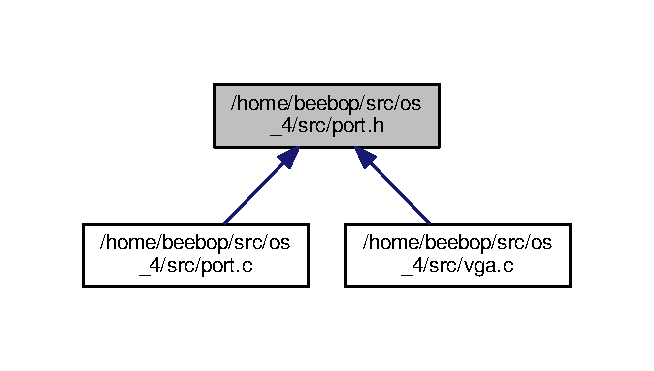
\includegraphics[width=314pt]{port_8h__dep__incl}
\end{center}
\end{figure}
\subsection*{Functions}
\begin{DoxyCompactItemize}
\item 
void \hyperlink{port_8h_a758def1b1168d2562f6e5030e343240a}{outb} (unsigned short port, unsigned char val)
\item 
void \hyperlink{port_8h_ab33f4442a8212007469ac760323d9d2a}{outw} (unsigned short port, unsigned short val)
\item 
unsigned char \hyperlink{port_8h_a8e267bc99eb4e47d1390903b8ea0e522}{inb} (unsigned short port)
\item 
unsigned short \hyperlink{port_8h_a6d87b47abf48abc5f8dbc9788b3e26a3}{inw} (unsigned short port)
\end{DoxyCompactItemize}


\subsection{Function Documentation}
\hypertarget{port_8h_a8e267bc99eb4e47d1390903b8ea0e522}{}\index{port.\+h@{port.\+h}!inb@{inb}}
\index{inb@{inb}!port.\+h@{port.\+h}}
\subsubsection[{inb}]{\setlength{\rightskip}{0pt plus 5cm}unsigned char inb (
\begin{DoxyParamCaption}
\item[{unsigned short}]{port}
\end{DoxyParamCaption}
)}\label{port_8h_a8e267bc99eb4e47d1390903b8ea0e522}
Reads one byte from a port. 
\begin{DoxyParams}[1]{Parameters}
\mbox{\tt in}  & {\em port} & The port to read from. \\
\hline
\end{DoxyParams}
\begin{DoxyReturn}{Returns}
The byte read from the port. 
\end{DoxyReturn}
\hypertarget{port_8h_a6d87b47abf48abc5f8dbc9788b3e26a3}{}\index{port.\+h@{port.\+h}!inw@{inw}}
\index{inw@{inw}!port.\+h@{port.\+h}}
\subsubsection[{inw}]{\setlength{\rightskip}{0pt plus 5cm}unsigned short inw (
\begin{DoxyParamCaption}
\item[{unsigned short}]{port}
\end{DoxyParamCaption}
)}\label{port_8h_a6d87b47abf48abc5f8dbc9788b3e26a3}
Reads one word from a port. 
\begin{DoxyParams}[1]{Parameters}
\mbox{\tt in}  & {\em port} & The port to read from. \\
\hline
\end{DoxyParams}
\begin{DoxyReturn}{Returns}
The word read from the port. 
\end{DoxyReturn}
\hypertarget{port_8h_a758def1b1168d2562f6e5030e343240a}{}\index{port.\+h@{port.\+h}!outb@{outb}}
\index{outb@{outb}!port.\+h@{port.\+h}}
\subsubsection[{outb}]{\setlength{\rightskip}{0pt plus 5cm}void outb (
\begin{DoxyParamCaption}
\item[{unsigned short}]{port, }
\item[{unsigned char}]{val}
\end{DoxyParamCaption}
)}\label{port_8h_a758def1b1168d2562f6e5030e343240a}
Writes one byte to a port. 
\begin{DoxyParams}[1]{Parameters}
\mbox{\tt in}  & {\em port} & The port to write to. \\
\hline
\mbox{\tt in}  & {\em val} & The byte to emit. \\
\hline
\end{DoxyParams}
\hypertarget{port_8h_ab33f4442a8212007469ac760323d9d2a}{}\index{port.\+h@{port.\+h}!outw@{outw}}
\index{outw@{outw}!port.\+h@{port.\+h}}
\subsubsection[{outw}]{\setlength{\rightskip}{0pt plus 5cm}void outw (
\begin{DoxyParamCaption}
\item[{unsigned short}]{port, }
\item[{unsigned short}]{val}
\end{DoxyParamCaption}
)}\label{port_8h_ab33f4442a8212007469ac760323d9d2a}
Writes one word (2 bytes) to a port. 
\begin{DoxyParams}[1]{Parameters}
\mbox{\tt in}  & {\em port} & The port to write to. \\
\hline
\mbox{\tt in}  & {\em val} & The word to emit. \\
\hline
\end{DoxyParams}

\hypertarget{version_8h}{}\section{/home/beebop/src/os\+\_\+4/src/version.h File Reference}
\label{version_8h}\index{/home/beebop/src/os\+\_\+4/src/version.\+h@{/home/beebop/src/os\+\_\+4/src/version.\+h}}
This graph shows which files directly or indirectly include this file\+:
\nopagebreak
\begin{figure}[H]
\begin{center}
\leavevmode
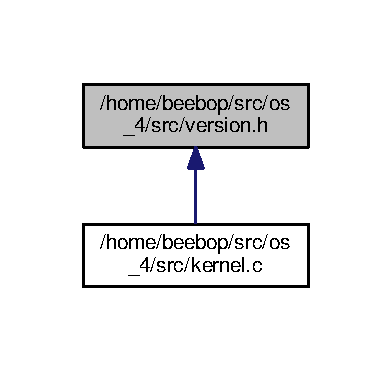
\includegraphics[width=188pt]{version_8h__dep__incl}
\end{center}
\end{figure}
\subsection*{Macros}
\begin{DoxyCompactItemize}
\item 
\#define \hyperlink{version_8h_a1c6d5de492ac61ad29aec7aa9a436bbf}{V\+E\+R\+S\+I\+O\+N}~\char`\"{}v0.\+1a/1 (git-\/c8041dc)\char`\"{}
\end{DoxyCompactItemize}


\subsection{Macro Definition Documentation}
\hypertarget{version_8h_a1c6d5de492ac61ad29aec7aa9a436bbf}{}\index{version.\+h@{version.\+h}!V\+E\+R\+S\+I\+O\+N@{V\+E\+R\+S\+I\+O\+N}}
\index{V\+E\+R\+S\+I\+O\+N@{V\+E\+R\+S\+I\+O\+N}!version.\+h@{version.\+h}}
\subsubsection[{V\+E\+R\+S\+I\+O\+N}]{\setlength{\rightskip}{0pt plus 5cm}\#define V\+E\+R\+S\+I\+O\+N~\char`\"{}v0.\+1a/1 (git-\/c8041dc)\char`\"{}}\label{version_8h_a1c6d5de492ac61ad29aec7aa9a436bbf}

\hypertarget{vga_8c}{}\section{/home/beebop/src/os\+\_\+4/src/vga.c File Reference}
\label{vga_8c}\index{/home/beebop/src/os\+\_\+4/src/vga.\+c@{/home/beebop/src/os\+\_\+4/src/vga.\+c}}
{\ttfamily \#include \char`\"{}vga.\+h\char`\"{}}\\*
{\ttfamily \#include \char`\"{}port.\+h\char`\"{}}\\*
Include dependency graph for vga.\+c\+:\nopagebreak
\begin{figure}[H]
\begin{center}
\leavevmode
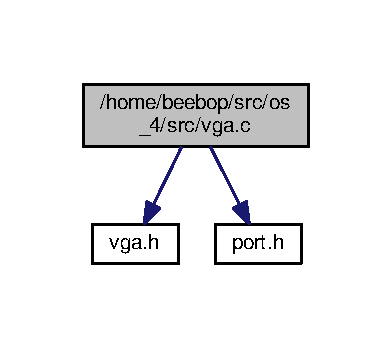
\includegraphics[width=188pt]{vga_8c__incl}
\end{center}
\end{figure}
\subsection*{Functions}
\begin{DoxyCompactItemize}
\item 
void \hyperlink{vga_8c_adef84c325b6265f4d05f439987eab121}{init\+\_\+vga} (void)
\item 
void \hyperlink{vga_8c_a42459dac9039d9b2c44b2c535969eeb0}{vga\+\_\+write\+\_\+reg} (unsigned short port, unsigned char idx, unsigned char dat)
\end{DoxyCompactItemize}


\subsection{Function Documentation}
\hypertarget{vga_8c_adef84c325b6265f4d05f439987eab121}{}\index{vga.\+c@{vga.\+c}!init\+\_\+vga@{init\+\_\+vga}}
\index{init\+\_\+vga@{init\+\_\+vga}!vga.\+c@{vga.\+c}}
\subsubsection[{init\+\_\+vga}]{\setlength{\rightskip}{0pt plus 5cm}void init\+\_\+vga (
\begin{DoxyParamCaption}
\item[{void}]{}
\end{DoxyParamCaption}
)}\label{vga_8c_adef84c325b6265f4d05f439987eab121}
Initialize the V\+G\+A subsystem and clear the screen. Currently initializes it in graphics mode. \hypertarget{vga_8c_a42459dac9039d9b2c44b2c535969eeb0}{}\index{vga.\+c@{vga.\+c}!vga\+\_\+write\+\_\+reg@{vga\+\_\+write\+\_\+reg}}
\index{vga\+\_\+write\+\_\+reg@{vga\+\_\+write\+\_\+reg}!vga.\+c@{vga.\+c}}
\subsubsection[{vga\+\_\+write\+\_\+reg}]{\setlength{\rightskip}{0pt plus 5cm}void vga\+\_\+write\+\_\+reg (
\begin{DoxyParamCaption}
\item[{unsigned short}]{port, }
\item[{unsigned char}]{idx, }
\item[{unsigned char}]{dat}
\end{DoxyParamCaption}
)}\label{vga_8c_a42459dac9039d9b2c44b2c535969eeb0}
Writes one byte to an indexed V\+G\+A register. 
\begin{DoxyParams}[1]{Parameters}
\mbox{\tt in}  & {\em port} & The base port of the register. \\
\hline
\mbox{\tt in}  & {\em idx} & The index of the V\+G\+A register. \\
\hline
\mbox{\tt in}  & {\em dat} & The data to write. \\
\hline
\end{DoxyParams}

\hypertarget{vga_8h}{}\section{/home/beebop/src/os\+\_\+4/src/vga.h File Reference}
\label{vga_8h}\index{/home/beebop/src/os\+\_\+4/src/vga.\+h@{/home/beebop/src/os\+\_\+4/src/vga.\+h}}
This graph shows which files directly or indirectly include this file\+:
\nopagebreak
\begin{figure}[H]
\begin{center}
\leavevmode
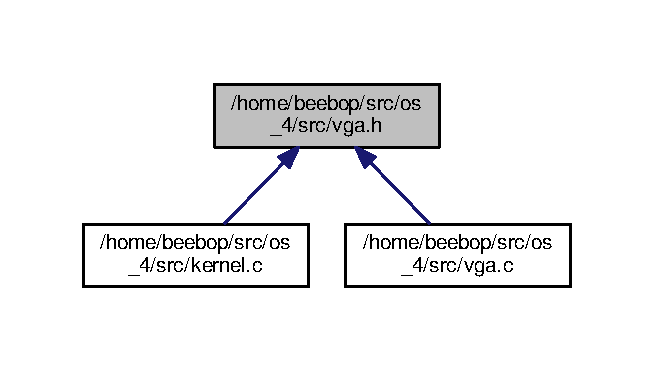
\includegraphics[width=350pt]{vga_8h__dep__incl}
\end{center}
\end{figure}
\subsection*{Macros}
\begin{DoxyCompactItemize}
\item 
\#define \hyperlink{vga_8h_ad61f065a3e0e7a7bd1525df3d15a6953}{N\+\_\+\+S\+E\+Q\+\_\+\+I\+D\+X}~5
\item 
\#define \hyperlink{vga_8h_a86301978523d49d2e15cd4c2d24f2b0d}{N\+\_\+\+C\+R\+T\+C\+\_\+\+I\+D\+X}~19
\item 
\#define \hyperlink{vga_8h_a377dfd92d57a796e5fd855cd1410ce42}{N\+\_\+\+G\+C\+\_\+\+I\+D\+X}~9
\item 
\#define \hyperlink{vga_8h_ae4c0ab86e3f36da5db686badfb28c52c}{N\+\_\+\+A\+T\+T\+R\+\_\+\+I\+D\+X}~15
\item 
\#define \hyperlink{vga_8h_acb0ac46e8f1bf7e9ce476914db9aa6ea}{V\+G\+A\+\_\+\+A\+T\+T\+R}~0x3\+C0
\item 
\#define \hyperlink{vga_8h_a634dc02903dec3173cfbfd9a5011f587}{V\+G\+A\+\_\+\+I\+D\+X\+\_\+\+R\+S\+T}~0x3\+D\+A
\item 
\#define \hyperlink{vga_8h_aaebe724fc2d035e37bef596584215260}{V\+G\+A\+\_\+\+M\+O\+R}~0x3\+C2
\item 
\#define \hyperlink{vga_8h_ad4c5bd530a03da9cb5aa105c9ceee573}{V\+G\+A\+\_\+\+M\+I\+R}~0x3\+C\+C
\item 
\#define \hyperlink{vga_8h_af7796c3fcfbb7182b15eda3709d7a432}{V\+G\+A\+\_\+\+S\+E\+Q}~0x3\+C4
\item 
\#define \hyperlink{vga_8h_a833ed8801d1eac123134d17dbbc82006}{V\+G\+A\+\_\+\+G\+C}~0x3\+C\+E
\item 
\#define \hyperlink{vga_8h_a70e51dbc2468cebf9b87ce7b2cbae708}{V\+G\+A\+\_\+\+C\+R\+T\+C}~0x3\+D4
\item 
\#define \hyperlink{vga_8h_a83a1104fbaf8794026d8ef5d84c651ef}{V\+G\+A\+\_\+\+D\+A\+C\+M\+A\+S\+K}~0x3\+C6
\item 
\#define \hyperlink{vga_8h_ae190246c8300bdebabaf41aa7b98de94}{V\+G\+A\+\_\+\+D\+A\+C1}~0x3\+C8
\item 
\#define \hyperlink{vga_8h_a74ae869daeda5575bd9cd4458e1d6f9c}{V\+G\+A\+\_\+\+D\+A\+C2}~0x3\+C9
\item 
\#define \hyperlink{vga_8h_a593c4720b0ab1f310cf71dc053885d19}{V\+G\+A\+\_\+\+D\+A\+C3}~0x3\+C7
\item 
\#define \hyperlink{vga_8h_af67d72f9e2eda7cecbb3acc5f826aaee}{A\+T\+T\+R\+\_\+\+M\+C\+T\+L}~0x10
\item 
\#define \hyperlink{vga_8h_adb56366965d8e44da81214dd86c9c3a3}{A\+T\+T\+R\+\_\+\+O\+S\+C\+N}~0x11
\item 
\#define \hyperlink{vga_8h_aadccf1d2a7e39e697ab456570b2b9625}{A\+T\+T\+R\+\_\+\+C\+P\+E}~0x12
\item 
\#define \hyperlink{vga_8h_af211be3eeb891d39bdccd3a1d3388c59}{A\+T\+T\+R\+\_\+\+H\+P\+A\+N}~0x13
\item 
\#define \hyperlink{vga_8h_a7529974b9122bd7040515749b00745da}{A\+T\+T\+R\+\_\+\+C\+S\+E\+L}~0x14
\item 
\#define \hyperlink{vga_8h_a4868042d04ed00f634b1886f3575f9a9}{S\+E\+Q\+\_\+\+R\+S\+T}~0x00
\item 
\#define \hyperlink{vga_8h_a7643c8112da9a6d965732aa4779eb026}{S\+E\+Q\+\_\+\+C\+M\+O\+D\+E}~0x01
\item 
\#define \hyperlink{vga_8h_abf109e2a8642ca8ea6f74d8cccd84898}{S\+E\+Q\+\_\+\+M\+M\+A\+S\+K}~0x02
\item 
\#define \hyperlink{vga_8h_a97a667f2e2866dcce41def4066459253}{S\+E\+Q\+\_\+\+C\+S\+E\+L}~0x03
\item 
\#define \hyperlink{vga_8h_a1e3d5d818670c09a987e14595b81d24b}{S\+E\+Q\+\_\+\+M\+M\+O\+D\+E}~0x04
\item 
\#define \hyperlink{vga_8h_ad9ad449f693e229a155e31c2b2e5d29b}{G\+C\+\_\+\+S\+E\+T\+\_\+\+R\+S\+T}~0x00
\item 
\#define \hyperlink{vga_8h_a816e6122661ce73da47b55ae4911a9a7}{G\+C\+\_\+\+E\+N\+\_\+\+S\+T\+\_\+\+R\+T}~0x01
\item 
\#define \hyperlink{vga_8h_a26e4d0698508a954ca30a285427caf86}{G\+C\+\_\+\+C\+O\+M\+P\+A\+R\+E}~0x02
\item 
\#define \hyperlink{vga_8h_a78b874928f3b2da7d3aba922e0360a37}{G\+C\+\_\+\+R\+O\+T\+A\+T\+E}~0x03
\item 
\#define \hyperlink{vga_8h_a905ca51e0e01d01c850b6200148f99d8}{G\+C\+\_\+\+M\+O\+D\+E}~0x05
\item 
\#define \hyperlink{vga_8h_ae7bf4ce899bee250a3a0ebe5e06cee19}{G\+C\+\_\+\+M\+I\+S\+C}~0x06
\item 
\#define \hyperlink{vga_8h_aedfe7e3a696381edff689f77ccced9e0}{G\+C\+\_\+\+B\+I\+T\+M\+A\+S\+K}~0x08
\item 
\#define \hyperlink{vga_8h_acbd413d7f16fed55ce7b6dca80f8094b}{C\+R\+T\+C\+\_\+\+H\+T\+O\+T\+A\+L}~0x00
\item 
\#define \hyperlink{vga_8h_a25ae64dd9457afa0314f3dfb9a6434e9}{C\+R\+T\+C\+\_\+\+H\+D\+E\+E}~0x01
\item 
\#define \hyperlink{vga_8h_af60ad0aa89abafef0b6c5f0d7a8ed5d5}{C\+R\+T\+C\+\_\+\+H\+B\+L\+S}~0x02
\item 
\#define \hyperlink{vga_8h_abbb33e888ffff1a4d435673e9ac34b7b}{C\+R\+T\+C\+\_\+\+H\+B\+L\+E}~0x03
\item 
\#define \hyperlink{vga_8h_a0d9cc090105731c77fa41a6c5f8a8f94}{C\+R\+T\+C\+\_\+\+H\+R\+T\+S}~0x04
\item 
\#define \hyperlink{vga_8h_abfe5222c90908c2b031be39434f0f612}{C\+R\+T\+C\+\_\+\+H\+R\+T\+E}~0x05
\item 
\#define \hyperlink{vga_8h_a096bbb3087184390dc4e46a78e7776d8}{C\+R\+T\+C\+\_\+\+V\+T\+O\+T\+A\+L}~0x06
\item 
\#define \hyperlink{vga_8h_a0ba498fec085fee19e0c99728e47c1f6}{C\+R\+T\+C\+\_\+\+O\+F\+R\+E\+G}~0x07
\item 
\#define \hyperlink{vga_8h_a1baf1b8464a763c694b6595c1b79ca7f}{C\+R\+T\+C\+\_\+\+P\+R\+S\+C\+A\+N}~0x08
\item 
\#define \hyperlink{vga_8h_a91594ce7c81441ac654bac1e0884e1a6}{C\+R\+T\+C\+\_\+\+M\+A\+X\+S\+C\+N}~0x09
\item 
\#define \hyperlink{vga_8h_ac3e8ca31f339a9f2b987326340cc721f}{C\+R\+T\+C\+\_\+\+V\+R\+T\+S}~0x10
\item 
\#define \hyperlink{vga_8h_a4875db97e7aa6895e251b71b0d9aea67}{C\+R\+T\+C\+\_\+\+V\+R\+T\+E}~0x11
\item 
\#define \hyperlink{vga_8h_a21965da476bfc0a677bccf6e50d191e7}{C\+R\+T\+C\+\_\+\+V\+D\+E\+E}~0x12
\item 
\#define \hyperlink{vga_8h_ac5de12adde1e7164bacb893849e83659}{C\+R\+T\+C\+\_\+\+L\+W\+I\+D\+T\+H}~0x13
\item 
\#define \hyperlink{vga_8h_a01ed24f49e638969b74180e0eb606af1}{C\+R\+T\+C\+\_\+\+U\+N\+D\+L\+O\+C}~0x14
\item 
\#define \hyperlink{vga_8h_aca57cdc7059066048f1d3a13ae49795d}{C\+R\+T\+C\+\_\+\+V\+B\+L\+S}~0x15
\item 
\#define \hyperlink{vga_8h_a243258a8e45628ea6f4d50a5522ea43b}{C\+R\+T\+C\+\_\+\+V\+B\+L\+E}~0x16
\item 
\#define \hyperlink{vga_8h_a72a035619a6a3afb9fc24105ab77dfb4}{C\+R\+T\+C\+\_\+\+M\+C\+T\+L}~0x17
\item 
\#define \hyperlink{vga_8h_a43f727238ef41c41ffa4ed00297b71a5}{M\+O\+R\+\_\+\+I\+O\+A\+S}~0x01
\item 
\#define \hyperlink{vga_8h_abbb8c671d93393a3979d892a4bf7869b}{M\+O\+R\+\_\+\+R\+A\+M\+E\+N}~0x02
\item 
\#define \hyperlink{vga_8h_a7e6c5567fae2613eb58a563332ccd097}{M\+O\+R\+\_\+\+C\+L\+O\+C\+K}(i)~(((i) \& 0x3) $<$$<$ 2)
\item 
\#define \hyperlink{vga_8h_a9dcac7eb26f1090a64af829460a447ba}{M\+O\+R\+\_\+\+O\+E\+P\+A\+G\+E}~0x20
\item 
\#define \hyperlink{vga_8h_a5ecb5b3d02c4c935aed76b5c3270b82f}{M\+O\+R\+\_\+\+H\+S\+Y\+N\+C\+P}~0x40
\item 
\#define \hyperlink{vga_8h_af226ad03f6e35487c7bc634129477364}{M\+O\+R\+\_\+\+V\+S\+Y\+N\+C\+P}~0x80
\item 
\#define \hyperlink{vga_8h_a4c7e63c99b310db6928789009bda3e28}{M\+C\+T\+L\+\_\+\+A\+T\+G\+E}~0x01
\item 
\#define \hyperlink{vga_8h_a9a0f5773ce5bfa92050afade160536fa}{M\+C\+T\+L\+\_\+\+M\+O\+N\+O}~0x02
\item 
\#define \hyperlink{vga_8h_a25dc415c8e004de709a46c98ae8216ef}{M\+C\+T\+L\+\_\+\+L\+G\+E}~0x04
\item 
\#define \hyperlink{vga_8h_a50ca7305d50314a5cc0f8e166206b922}{M\+C\+T\+L\+\_\+\+B\+L\+I\+N\+K}~0x08
\item 
\#define \hyperlink{vga_8h_abccfef2e69a62284552a498ec3e552d5}{M\+C\+T\+L\+\_\+\+P\+P\+M}~0x20
\item 
\#define \hyperlink{vga_8h_a590972bbe8a5f4dbfe408d2bb5f053e6}{M\+C\+T\+L\+\_\+8\+B\+I\+T}~0x40
\item 
\#define \hyperlink{vga_8h_a82b16928b54136bbce6a991872307565}{M\+C\+T\+L\+\_\+\+P54\+S}~0x80
\item 
\#define \hyperlink{vga_8h_add6cb20db5c6d930e75ee5e8a92d72f2}{R\+S\+T\+\_\+\+A\+S\+Y\+N\+C}~0x01
\item 
\#define \hyperlink{vga_8h_a843d3c1018976459ec6bcf555908da5c}{R\+S\+T\+\_\+\+S\+Y\+N\+C}~0x02
\item 
\#define \hyperlink{vga_8h_ab7aa98fe6737a410a896eacaca8e2919}{C\+M\+O\+D\+E\+\_\+98\+D\+M}~0x01
\item 
\#define \hyperlink{vga_8h_af77e7949af47e71bb4a07c9d1dfc6e5a}{C\+M\+O\+D\+E\+\_\+\+S\+L\+R}~0x04
\item 
\#define \hyperlink{vga_8h_ad0d84123842fb0beff42a53db717ff2d}{C\+M\+O\+D\+E\+\_\+\+D\+C\+R}~0x08
\item 
\#define \hyperlink{vga_8h_a11cb9bf20c9d6f8abeb7a99c01ff7c66}{C\+M\+O\+D\+E\+\_\+\+S4}~0x10
\item 
\#define \hyperlink{vga_8h_a06e34e9ee4952ef22a93f824d3bafd52}{C\+M\+O\+D\+E\+\_\+\+S\+D}~0x20
\item 
\#define \hyperlink{vga_8h_ad0b2d73aa98c5eb1c73f627e249588b3}{C\+S\+E\+L\+\_\+\+A}(i)~((((i) \& 0x03) $<$$<$ 2) $\vert$ (((i) \& 0x04) $<$$<$ 3))
\item 
\#define \hyperlink{vga_8h_a57101cbcde6a0b308e6f78d451b1d05a}{C\+S\+E\+L\+\_\+\+B}(i)~(((i) \& 0x03) $\vert$ (((i) \& 0x04) $<$$<$ 2))
\item 
\#define \hyperlink{vga_8h_ae524fc74fe3acde1c050bf0e84616626}{M\+M\+O\+D\+E\+\_\+\+E\+X\+T\+M}~0x02
\item 
\#define \hyperlink{vga_8h_a9924603882d01d7aff8895b39fb35979}{M\+M\+O\+D\+E\+\_\+\+O\+E}~0x04
\item 
\#define \hyperlink{vga_8h_a508d5b41af971997ca73156475f1a169}{M\+M\+O\+D\+E\+\_\+\+C\+H4}~0x08
\item 
\#define \hyperlink{vga_8h_a85cda99eab9022e29270a9bf095583bd}{M\+O\+D\+E\+\_\+\+W\+R\+I\+T\+E}(i)~((i) \& 0x03)
\item 
\#define \hyperlink{vga_8h_a0ac8b5ff52772ec706a05bfffd241ab2}{M\+O\+D\+E\+\_\+\+R\+E\+A\+D}(i)~((i) $<$$<$ 3)
\item 
\#define \hyperlink{vga_8h_a173ec59cbb4ba878f65ea0ac0999fd3e}{M\+O\+D\+E\+\_\+\+H\+O\+E}~0x10
\item 
\#define \hyperlink{vga_8h_a92f0bfcee023e8c8911da39387f8cee6}{M\+O\+D\+E\+\_\+\+S\+H\+R}~0x20
\item 
\#define \hyperlink{vga_8h_ae929377b61a15172a66c9b06844311fb}{M\+O\+D\+E\+\_\+\+S\+H256}~0x40
\item 
\#define \hyperlink{vga_8h_a1215cd18c0694c7ad5636f320fa9376c}{M\+I\+S\+C\+\_\+\+A\+D\+I\+S}~0x01
\item 
\#define \hyperlink{vga_8h_a8e45f298c73c336a913dde39a8e27091}{M\+I\+S\+C\+\_\+\+C\+H\+O\+E}~0x02
\item 
\#define \hyperlink{vga_8h_a9bcf1113f113b6065bb9dc1d606ab733}{M\+I\+S\+C\+\_\+\+M\+M\+A\+P}(i)~(((i) \& 0x03) $<$$<$ 2)
\item 
\#define \hyperlink{vga_8h_a83eb6ee44e7f506a2089981c91c38887}{R\+O\+T\+A\+T\+E\+\_\+\+C\+O\+U\+N\+T}(i)~((i) \& 0x03)
\item 
\#define \hyperlink{vga_8h_a1b755af4fec583854628df318f998c68}{R\+O\+T\+A\+T\+E\+\_\+\+I\+D\+E\+N\+T}~0x00
\item 
\#define \hyperlink{vga_8h_a8aea5cd51c72ebe76e3d20c6af2bfc6c}{R\+O\+T\+A\+T\+E\+\_\+\+A\+N\+D}~0x08
\item 
\#define \hyperlink{vga_8h_a8c3b53cf477fd7d402c555dfa10edbb5}{R\+O\+T\+A\+T\+E\+\_\+\+O\+R}~0x10
\item 
\#define \hyperlink{vga_8h_aaa03cdcbcf718d2aa76c4a6a2d9c6d85}{R\+O\+T\+A\+T\+E\+\_\+\+X\+O\+R}~0x18
\end{DoxyCompactItemize}
\subsection*{Functions}
\begin{DoxyCompactItemize}
\item 
void \hyperlink{vga_8h_adef84c325b6265f4d05f439987eab121}{init\+\_\+vga} (void)
\item 
void \hyperlink{vga_8h_a42459dac9039d9b2c44b2c535969eeb0}{vga\+\_\+write\+\_\+reg} (unsigned short port, unsigned char idx, unsigned char dat)
\item 
void \hyperlink{vga_8h_a8122db7ab751f5409cb3e94b102364b5}{vga\+\_\+write\+\_\+pix} (int x, int y, int color)
\item 
void \hyperlink{vga_8h_ab88b680bc59f7446af3e5b97961f1c27}{vga\+\_\+set\+\_\+palette} (int idx, unsigned char r, unsigned char g, unsigned char b)
\item 
void \hyperlink{vga_8h_a0a09bc3b0111af74c7aa94b6504c3e9b}{vga\+\_\+clear} ()
\end{DoxyCompactItemize}


\subsection{Macro Definition Documentation}
\hypertarget{vga_8h_aadccf1d2a7e39e697ab456570b2b9625}{}\index{vga.\+h@{vga.\+h}!A\+T\+T\+R\+\_\+\+C\+P\+E@{A\+T\+T\+R\+\_\+\+C\+P\+E}}
\index{A\+T\+T\+R\+\_\+\+C\+P\+E@{A\+T\+T\+R\+\_\+\+C\+P\+E}!vga.\+h@{vga.\+h}}
\subsubsection[{A\+T\+T\+R\+\_\+\+C\+P\+E}]{\setlength{\rightskip}{0pt plus 5cm}\#define A\+T\+T\+R\+\_\+\+C\+P\+E~0x12}\label{vga_8h_aadccf1d2a7e39e697ab456570b2b9625}
\hypertarget{vga_8h_a7529974b9122bd7040515749b00745da}{}\index{vga.\+h@{vga.\+h}!A\+T\+T\+R\+\_\+\+C\+S\+E\+L@{A\+T\+T\+R\+\_\+\+C\+S\+E\+L}}
\index{A\+T\+T\+R\+\_\+\+C\+S\+E\+L@{A\+T\+T\+R\+\_\+\+C\+S\+E\+L}!vga.\+h@{vga.\+h}}
\subsubsection[{A\+T\+T\+R\+\_\+\+C\+S\+E\+L}]{\setlength{\rightskip}{0pt plus 5cm}\#define A\+T\+T\+R\+\_\+\+C\+S\+E\+L~0x14}\label{vga_8h_a7529974b9122bd7040515749b00745da}
\hypertarget{vga_8h_af211be3eeb891d39bdccd3a1d3388c59}{}\index{vga.\+h@{vga.\+h}!A\+T\+T\+R\+\_\+\+H\+P\+A\+N@{A\+T\+T\+R\+\_\+\+H\+P\+A\+N}}
\index{A\+T\+T\+R\+\_\+\+H\+P\+A\+N@{A\+T\+T\+R\+\_\+\+H\+P\+A\+N}!vga.\+h@{vga.\+h}}
\subsubsection[{A\+T\+T\+R\+\_\+\+H\+P\+A\+N}]{\setlength{\rightskip}{0pt plus 5cm}\#define A\+T\+T\+R\+\_\+\+H\+P\+A\+N~0x13}\label{vga_8h_af211be3eeb891d39bdccd3a1d3388c59}
\hypertarget{vga_8h_af67d72f9e2eda7cecbb3acc5f826aaee}{}\index{vga.\+h@{vga.\+h}!A\+T\+T\+R\+\_\+\+M\+C\+T\+L@{A\+T\+T\+R\+\_\+\+M\+C\+T\+L}}
\index{A\+T\+T\+R\+\_\+\+M\+C\+T\+L@{A\+T\+T\+R\+\_\+\+M\+C\+T\+L}!vga.\+h@{vga.\+h}}
\subsubsection[{A\+T\+T\+R\+\_\+\+M\+C\+T\+L}]{\setlength{\rightskip}{0pt plus 5cm}\#define A\+T\+T\+R\+\_\+\+M\+C\+T\+L~0x10}\label{vga_8h_af67d72f9e2eda7cecbb3acc5f826aaee}
\hypertarget{vga_8h_adb56366965d8e44da81214dd86c9c3a3}{}\index{vga.\+h@{vga.\+h}!A\+T\+T\+R\+\_\+\+O\+S\+C\+N@{A\+T\+T\+R\+\_\+\+O\+S\+C\+N}}
\index{A\+T\+T\+R\+\_\+\+O\+S\+C\+N@{A\+T\+T\+R\+\_\+\+O\+S\+C\+N}!vga.\+h@{vga.\+h}}
\subsubsection[{A\+T\+T\+R\+\_\+\+O\+S\+C\+N}]{\setlength{\rightskip}{0pt plus 5cm}\#define A\+T\+T\+R\+\_\+\+O\+S\+C\+N~0x11}\label{vga_8h_adb56366965d8e44da81214dd86c9c3a3}
\hypertarget{vga_8h_ab7aa98fe6737a410a896eacaca8e2919}{}\index{vga.\+h@{vga.\+h}!C\+M\+O\+D\+E\+\_\+98\+D\+M@{C\+M\+O\+D\+E\+\_\+98\+D\+M}}
\index{C\+M\+O\+D\+E\+\_\+98\+D\+M@{C\+M\+O\+D\+E\+\_\+98\+D\+M}!vga.\+h@{vga.\+h}}
\subsubsection[{C\+M\+O\+D\+E\+\_\+98\+D\+M}]{\setlength{\rightskip}{0pt plus 5cm}\#define C\+M\+O\+D\+E\+\_\+98\+D\+M~0x01}\label{vga_8h_ab7aa98fe6737a410a896eacaca8e2919}
\hypertarget{vga_8h_ad0d84123842fb0beff42a53db717ff2d}{}\index{vga.\+h@{vga.\+h}!C\+M\+O\+D\+E\+\_\+\+D\+C\+R@{C\+M\+O\+D\+E\+\_\+\+D\+C\+R}}
\index{C\+M\+O\+D\+E\+\_\+\+D\+C\+R@{C\+M\+O\+D\+E\+\_\+\+D\+C\+R}!vga.\+h@{vga.\+h}}
\subsubsection[{C\+M\+O\+D\+E\+\_\+\+D\+C\+R}]{\setlength{\rightskip}{0pt plus 5cm}\#define C\+M\+O\+D\+E\+\_\+\+D\+C\+R~0x08}\label{vga_8h_ad0d84123842fb0beff42a53db717ff2d}
\hypertarget{vga_8h_a11cb9bf20c9d6f8abeb7a99c01ff7c66}{}\index{vga.\+h@{vga.\+h}!C\+M\+O\+D\+E\+\_\+\+S4@{C\+M\+O\+D\+E\+\_\+\+S4}}
\index{C\+M\+O\+D\+E\+\_\+\+S4@{C\+M\+O\+D\+E\+\_\+\+S4}!vga.\+h@{vga.\+h}}
\subsubsection[{C\+M\+O\+D\+E\+\_\+\+S4}]{\setlength{\rightskip}{0pt plus 5cm}\#define C\+M\+O\+D\+E\+\_\+\+S4~0x10}\label{vga_8h_a11cb9bf20c9d6f8abeb7a99c01ff7c66}
\hypertarget{vga_8h_a06e34e9ee4952ef22a93f824d3bafd52}{}\index{vga.\+h@{vga.\+h}!C\+M\+O\+D\+E\+\_\+\+S\+D@{C\+M\+O\+D\+E\+\_\+\+S\+D}}
\index{C\+M\+O\+D\+E\+\_\+\+S\+D@{C\+M\+O\+D\+E\+\_\+\+S\+D}!vga.\+h@{vga.\+h}}
\subsubsection[{C\+M\+O\+D\+E\+\_\+\+S\+D}]{\setlength{\rightskip}{0pt plus 5cm}\#define C\+M\+O\+D\+E\+\_\+\+S\+D~0x20}\label{vga_8h_a06e34e9ee4952ef22a93f824d3bafd52}
\hypertarget{vga_8h_af77e7949af47e71bb4a07c9d1dfc6e5a}{}\index{vga.\+h@{vga.\+h}!C\+M\+O\+D\+E\+\_\+\+S\+L\+R@{C\+M\+O\+D\+E\+\_\+\+S\+L\+R}}
\index{C\+M\+O\+D\+E\+\_\+\+S\+L\+R@{C\+M\+O\+D\+E\+\_\+\+S\+L\+R}!vga.\+h@{vga.\+h}}
\subsubsection[{C\+M\+O\+D\+E\+\_\+\+S\+L\+R}]{\setlength{\rightskip}{0pt plus 5cm}\#define C\+M\+O\+D\+E\+\_\+\+S\+L\+R~0x04}\label{vga_8h_af77e7949af47e71bb4a07c9d1dfc6e5a}
\hypertarget{vga_8h_abbb33e888ffff1a4d435673e9ac34b7b}{}\index{vga.\+h@{vga.\+h}!C\+R\+T\+C\+\_\+\+H\+B\+L\+E@{C\+R\+T\+C\+\_\+\+H\+B\+L\+E}}
\index{C\+R\+T\+C\+\_\+\+H\+B\+L\+E@{C\+R\+T\+C\+\_\+\+H\+B\+L\+E}!vga.\+h@{vga.\+h}}
\subsubsection[{C\+R\+T\+C\+\_\+\+H\+B\+L\+E}]{\setlength{\rightskip}{0pt plus 5cm}\#define C\+R\+T\+C\+\_\+\+H\+B\+L\+E~0x03}\label{vga_8h_abbb33e888ffff1a4d435673e9ac34b7b}
\hypertarget{vga_8h_af60ad0aa89abafef0b6c5f0d7a8ed5d5}{}\index{vga.\+h@{vga.\+h}!C\+R\+T\+C\+\_\+\+H\+B\+L\+S@{C\+R\+T\+C\+\_\+\+H\+B\+L\+S}}
\index{C\+R\+T\+C\+\_\+\+H\+B\+L\+S@{C\+R\+T\+C\+\_\+\+H\+B\+L\+S}!vga.\+h@{vga.\+h}}
\subsubsection[{C\+R\+T\+C\+\_\+\+H\+B\+L\+S}]{\setlength{\rightskip}{0pt plus 5cm}\#define C\+R\+T\+C\+\_\+\+H\+B\+L\+S~0x02}\label{vga_8h_af60ad0aa89abafef0b6c5f0d7a8ed5d5}
\hypertarget{vga_8h_a25ae64dd9457afa0314f3dfb9a6434e9}{}\index{vga.\+h@{vga.\+h}!C\+R\+T\+C\+\_\+\+H\+D\+E\+E@{C\+R\+T\+C\+\_\+\+H\+D\+E\+E}}
\index{C\+R\+T\+C\+\_\+\+H\+D\+E\+E@{C\+R\+T\+C\+\_\+\+H\+D\+E\+E}!vga.\+h@{vga.\+h}}
\subsubsection[{C\+R\+T\+C\+\_\+\+H\+D\+E\+E}]{\setlength{\rightskip}{0pt plus 5cm}\#define C\+R\+T\+C\+\_\+\+H\+D\+E\+E~0x01}\label{vga_8h_a25ae64dd9457afa0314f3dfb9a6434e9}
\hypertarget{vga_8h_abfe5222c90908c2b031be39434f0f612}{}\index{vga.\+h@{vga.\+h}!C\+R\+T\+C\+\_\+\+H\+R\+T\+E@{C\+R\+T\+C\+\_\+\+H\+R\+T\+E}}
\index{C\+R\+T\+C\+\_\+\+H\+R\+T\+E@{C\+R\+T\+C\+\_\+\+H\+R\+T\+E}!vga.\+h@{vga.\+h}}
\subsubsection[{C\+R\+T\+C\+\_\+\+H\+R\+T\+E}]{\setlength{\rightskip}{0pt plus 5cm}\#define C\+R\+T\+C\+\_\+\+H\+R\+T\+E~0x05}\label{vga_8h_abfe5222c90908c2b031be39434f0f612}
\hypertarget{vga_8h_a0d9cc090105731c77fa41a6c5f8a8f94}{}\index{vga.\+h@{vga.\+h}!C\+R\+T\+C\+\_\+\+H\+R\+T\+S@{C\+R\+T\+C\+\_\+\+H\+R\+T\+S}}
\index{C\+R\+T\+C\+\_\+\+H\+R\+T\+S@{C\+R\+T\+C\+\_\+\+H\+R\+T\+S}!vga.\+h@{vga.\+h}}
\subsubsection[{C\+R\+T\+C\+\_\+\+H\+R\+T\+S}]{\setlength{\rightskip}{0pt plus 5cm}\#define C\+R\+T\+C\+\_\+\+H\+R\+T\+S~0x04}\label{vga_8h_a0d9cc090105731c77fa41a6c5f8a8f94}
\hypertarget{vga_8h_acbd413d7f16fed55ce7b6dca80f8094b}{}\index{vga.\+h@{vga.\+h}!C\+R\+T\+C\+\_\+\+H\+T\+O\+T\+A\+L@{C\+R\+T\+C\+\_\+\+H\+T\+O\+T\+A\+L}}
\index{C\+R\+T\+C\+\_\+\+H\+T\+O\+T\+A\+L@{C\+R\+T\+C\+\_\+\+H\+T\+O\+T\+A\+L}!vga.\+h@{vga.\+h}}
\subsubsection[{C\+R\+T\+C\+\_\+\+H\+T\+O\+T\+A\+L}]{\setlength{\rightskip}{0pt plus 5cm}\#define C\+R\+T\+C\+\_\+\+H\+T\+O\+T\+A\+L~0x00}\label{vga_8h_acbd413d7f16fed55ce7b6dca80f8094b}
\hypertarget{vga_8h_ac5de12adde1e7164bacb893849e83659}{}\index{vga.\+h@{vga.\+h}!C\+R\+T\+C\+\_\+\+L\+W\+I\+D\+T\+H@{C\+R\+T\+C\+\_\+\+L\+W\+I\+D\+T\+H}}
\index{C\+R\+T\+C\+\_\+\+L\+W\+I\+D\+T\+H@{C\+R\+T\+C\+\_\+\+L\+W\+I\+D\+T\+H}!vga.\+h@{vga.\+h}}
\subsubsection[{C\+R\+T\+C\+\_\+\+L\+W\+I\+D\+T\+H}]{\setlength{\rightskip}{0pt plus 5cm}\#define C\+R\+T\+C\+\_\+\+L\+W\+I\+D\+T\+H~0x13}\label{vga_8h_ac5de12adde1e7164bacb893849e83659}
\hypertarget{vga_8h_a91594ce7c81441ac654bac1e0884e1a6}{}\index{vga.\+h@{vga.\+h}!C\+R\+T\+C\+\_\+\+M\+A\+X\+S\+C\+N@{C\+R\+T\+C\+\_\+\+M\+A\+X\+S\+C\+N}}
\index{C\+R\+T\+C\+\_\+\+M\+A\+X\+S\+C\+N@{C\+R\+T\+C\+\_\+\+M\+A\+X\+S\+C\+N}!vga.\+h@{vga.\+h}}
\subsubsection[{C\+R\+T\+C\+\_\+\+M\+A\+X\+S\+C\+N}]{\setlength{\rightskip}{0pt plus 5cm}\#define C\+R\+T\+C\+\_\+\+M\+A\+X\+S\+C\+N~0x09}\label{vga_8h_a91594ce7c81441ac654bac1e0884e1a6}
\hypertarget{vga_8h_a72a035619a6a3afb9fc24105ab77dfb4}{}\index{vga.\+h@{vga.\+h}!C\+R\+T\+C\+\_\+\+M\+C\+T\+L@{C\+R\+T\+C\+\_\+\+M\+C\+T\+L}}
\index{C\+R\+T\+C\+\_\+\+M\+C\+T\+L@{C\+R\+T\+C\+\_\+\+M\+C\+T\+L}!vga.\+h@{vga.\+h}}
\subsubsection[{C\+R\+T\+C\+\_\+\+M\+C\+T\+L}]{\setlength{\rightskip}{0pt plus 5cm}\#define C\+R\+T\+C\+\_\+\+M\+C\+T\+L~0x17}\label{vga_8h_a72a035619a6a3afb9fc24105ab77dfb4}
\hypertarget{vga_8h_a0ba498fec085fee19e0c99728e47c1f6}{}\index{vga.\+h@{vga.\+h}!C\+R\+T\+C\+\_\+\+O\+F\+R\+E\+G@{C\+R\+T\+C\+\_\+\+O\+F\+R\+E\+G}}
\index{C\+R\+T\+C\+\_\+\+O\+F\+R\+E\+G@{C\+R\+T\+C\+\_\+\+O\+F\+R\+E\+G}!vga.\+h@{vga.\+h}}
\subsubsection[{C\+R\+T\+C\+\_\+\+O\+F\+R\+E\+G}]{\setlength{\rightskip}{0pt plus 5cm}\#define C\+R\+T\+C\+\_\+\+O\+F\+R\+E\+G~0x07}\label{vga_8h_a0ba498fec085fee19e0c99728e47c1f6}
\hypertarget{vga_8h_a1baf1b8464a763c694b6595c1b79ca7f}{}\index{vga.\+h@{vga.\+h}!C\+R\+T\+C\+\_\+\+P\+R\+S\+C\+A\+N@{C\+R\+T\+C\+\_\+\+P\+R\+S\+C\+A\+N}}
\index{C\+R\+T\+C\+\_\+\+P\+R\+S\+C\+A\+N@{C\+R\+T\+C\+\_\+\+P\+R\+S\+C\+A\+N}!vga.\+h@{vga.\+h}}
\subsubsection[{C\+R\+T\+C\+\_\+\+P\+R\+S\+C\+A\+N}]{\setlength{\rightskip}{0pt plus 5cm}\#define C\+R\+T\+C\+\_\+\+P\+R\+S\+C\+A\+N~0x08}\label{vga_8h_a1baf1b8464a763c694b6595c1b79ca7f}
\hypertarget{vga_8h_a01ed24f49e638969b74180e0eb606af1}{}\index{vga.\+h@{vga.\+h}!C\+R\+T\+C\+\_\+\+U\+N\+D\+L\+O\+C@{C\+R\+T\+C\+\_\+\+U\+N\+D\+L\+O\+C}}
\index{C\+R\+T\+C\+\_\+\+U\+N\+D\+L\+O\+C@{C\+R\+T\+C\+\_\+\+U\+N\+D\+L\+O\+C}!vga.\+h@{vga.\+h}}
\subsubsection[{C\+R\+T\+C\+\_\+\+U\+N\+D\+L\+O\+C}]{\setlength{\rightskip}{0pt plus 5cm}\#define C\+R\+T\+C\+\_\+\+U\+N\+D\+L\+O\+C~0x14}\label{vga_8h_a01ed24f49e638969b74180e0eb606af1}
\hypertarget{vga_8h_a243258a8e45628ea6f4d50a5522ea43b}{}\index{vga.\+h@{vga.\+h}!C\+R\+T\+C\+\_\+\+V\+B\+L\+E@{C\+R\+T\+C\+\_\+\+V\+B\+L\+E}}
\index{C\+R\+T\+C\+\_\+\+V\+B\+L\+E@{C\+R\+T\+C\+\_\+\+V\+B\+L\+E}!vga.\+h@{vga.\+h}}
\subsubsection[{C\+R\+T\+C\+\_\+\+V\+B\+L\+E}]{\setlength{\rightskip}{0pt plus 5cm}\#define C\+R\+T\+C\+\_\+\+V\+B\+L\+E~0x16}\label{vga_8h_a243258a8e45628ea6f4d50a5522ea43b}
\hypertarget{vga_8h_aca57cdc7059066048f1d3a13ae49795d}{}\index{vga.\+h@{vga.\+h}!C\+R\+T\+C\+\_\+\+V\+B\+L\+S@{C\+R\+T\+C\+\_\+\+V\+B\+L\+S}}
\index{C\+R\+T\+C\+\_\+\+V\+B\+L\+S@{C\+R\+T\+C\+\_\+\+V\+B\+L\+S}!vga.\+h@{vga.\+h}}
\subsubsection[{C\+R\+T\+C\+\_\+\+V\+B\+L\+S}]{\setlength{\rightskip}{0pt plus 5cm}\#define C\+R\+T\+C\+\_\+\+V\+B\+L\+S~0x15}\label{vga_8h_aca57cdc7059066048f1d3a13ae49795d}
\hypertarget{vga_8h_a21965da476bfc0a677bccf6e50d191e7}{}\index{vga.\+h@{vga.\+h}!C\+R\+T\+C\+\_\+\+V\+D\+E\+E@{C\+R\+T\+C\+\_\+\+V\+D\+E\+E}}
\index{C\+R\+T\+C\+\_\+\+V\+D\+E\+E@{C\+R\+T\+C\+\_\+\+V\+D\+E\+E}!vga.\+h@{vga.\+h}}
\subsubsection[{C\+R\+T\+C\+\_\+\+V\+D\+E\+E}]{\setlength{\rightskip}{0pt plus 5cm}\#define C\+R\+T\+C\+\_\+\+V\+D\+E\+E~0x12}\label{vga_8h_a21965da476bfc0a677bccf6e50d191e7}
\hypertarget{vga_8h_a4875db97e7aa6895e251b71b0d9aea67}{}\index{vga.\+h@{vga.\+h}!C\+R\+T\+C\+\_\+\+V\+R\+T\+E@{C\+R\+T\+C\+\_\+\+V\+R\+T\+E}}
\index{C\+R\+T\+C\+\_\+\+V\+R\+T\+E@{C\+R\+T\+C\+\_\+\+V\+R\+T\+E}!vga.\+h@{vga.\+h}}
\subsubsection[{C\+R\+T\+C\+\_\+\+V\+R\+T\+E}]{\setlength{\rightskip}{0pt plus 5cm}\#define C\+R\+T\+C\+\_\+\+V\+R\+T\+E~0x11}\label{vga_8h_a4875db97e7aa6895e251b71b0d9aea67}
\hypertarget{vga_8h_ac3e8ca31f339a9f2b987326340cc721f}{}\index{vga.\+h@{vga.\+h}!C\+R\+T\+C\+\_\+\+V\+R\+T\+S@{C\+R\+T\+C\+\_\+\+V\+R\+T\+S}}
\index{C\+R\+T\+C\+\_\+\+V\+R\+T\+S@{C\+R\+T\+C\+\_\+\+V\+R\+T\+S}!vga.\+h@{vga.\+h}}
\subsubsection[{C\+R\+T\+C\+\_\+\+V\+R\+T\+S}]{\setlength{\rightskip}{0pt plus 5cm}\#define C\+R\+T\+C\+\_\+\+V\+R\+T\+S~0x10}\label{vga_8h_ac3e8ca31f339a9f2b987326340cc721f}
\hypertarget{vga_8h_a096bbb3087184390dc4e46a78e7776d8}{}\index{vga.\+h@{vga.\+h}!C\+R\+T\+C\+\_\+\+V\+T\+O\+T\+A\+L@{C\+R\+T\+C\+\_\+\+V\+T\+O\+T\+A\+L}}
\index{C\+R\+T\+C\+\_\+\+V\+T\+O\+T\+A\+L@{C\+R\+T\+C\+\_\+\+V\+T\+O\+T\+A\+L}!vga.\+h@{vga.\+h}}
\subsubsection[{C\+R\+T\+C\+\_\+\+V\+T\+O\+T\+A\+L}]{\setlength{\rightskip}{0pt plus 5cm}\#define C\+R\+T\+C\+\_\+\+V\+T\+O\+T\+A\+L~0x06}\label{vga_8h_a096bbb3087184390dc4e46a78e7776d8}
\hypertarget{vga_8h_ad0b2d73aa98c5eb1c73f627e249588b3}{}\index{vga.\+h@{vga.\+h}!C\+S\+E\+L\+\_\+\+A@{C\+S\+E\+L\+\_\+\+A}}
\index{C\+S\+E\+L\+\_\+\+A@{C\+S\+E\+L\+\_\+\+A}!vga.\+h@{vga.\+h}}
\subsubsection[{C\+S\+E\+L\+\_\+\+A}]{\setlength{\rightskip}{0pt plus 5cm}\#define C\+S\+E\+L\+\_\+\+A(
\begin{DoxyParamCaption}
\item[{}]{i}
\end{DoxyParamCaption}
)~((((i) \& 0x03) $<$$<$ 2) $\vert$ (((i) \& 0x04) $<$$<$ 3))}\label{vga_8h_ad0b2d73aa98c5eb1c73f627e249588b3}
\hypertarget{vga_8h_a57101cbcde6a0b308e6f78d451b1d05a}{}\index{vga.\+h@{vga.\+h}!C\+S\+E\+L\+\_\+\+B@{C\+S\+E\+L\+\_\+\+B}}
\index{C\+S\+E\+L\+\_\+\+B@{C\+S\+E\+L\+\_\+\+B}!vga.\+h@{vga.\+h}}
\subsubsection[{C\+S\+E\+L\+\_\+\+B}]{\setlength{\rightskip}{0pt plus 5cm}\#define C\+S\+E\+L\+\_\+\+B(
\begin{DoxyParamCaption}
\item[{}]{i}
\end{DoxyParamCaption}
)~(((i) \& 0x03) $\vert$ (((i) \& 0x04) $<$$<$ 2))}\label{vga_8h_a57101cbcde6a0b308e6f78d451b1d05a}
\hypertarget{vga_8h_aedfe7e3a696381edff689f77ccced9e0}{}\index{vga.\+h@{vga.\+h}!G\+C\+\_\+\+B\+I\+T\+M\+A\+S\+K@{G\+C\+\_\+\+B\+I\+T\+M\+A\+S\+K}}
\index{G\+C\+\_\+\+B\+I\+T\+M\+A\+S\+K@{G\+C\+\_\+\+B\+I\+T\+M\+A\+S\+K}!vga.\+h@{vga.\+h}}
\subsubsection[{G\+C\+\_\+\+B\+I\+T\+M\+A\+S\+K}]{\setlength{\rightskip}{0pt plus 5cm}\#define G\+C\+\_\+\+B\+I\+T\+M\+A\+S\+K~0x08}\label{vga_8h_aedfe7e3a696381edff689f77ccced9e0}
\hypertarget{vga_8h_a26e4d0698508a954ca30a285427caf86}{}\index{vga.\+h@{vga.\+h}!G\+C\+\_\+\+C\+O\+M\+P\+A\+R\+E@{G\+C\+\_\+\+C\+O\+M\+P\+A\+R\+E}}
\index{G\+C\+\_\+\+C\+O\+M\+P\+A\+R\+E@{G\+C\+\_\+\+C\+O\+M\+P\+A\+R\+E}!vga.\+h@{vga.\+h}}
\subsubsection[{G\+C\+\_\+\+C\+O\+M\+P\+A\+R\+E}]{\setlength{\rightskip}{0pt plus 5cm}\#define G\+C\+\_\+\+C\+O\+M\+P\+A\+R\+E~0x02}\label{vga_8h_a26e4d0698508a954ca30a285427caf86}
\hypertarget{vga_8h_a816e6122661ce73da47b55ae4911a9a7}{}\index{vga.\+h@{vga.\+h}!G\+C\+\_\+\+E\+N\+\_\+\+S\+T\+\_\+\+R\+T@{G\+C\+\_\+\+E\+N\+\_\+\+S\+T\+\_\+\+R\+T}}
\index{G\+C\+\_\+\+E\+N\+\_\+\+S\+T\+\_\+\+R\+T@{G\+C\+\_\+\+E\+N\+\_\+\+S\+T\+\_\+\+R\+T}!vga.\+h@{vga.\+h}}
\subsubsection[{G\+C\+\_\+\+E\+N\+\_\+\+S\+T\+\_\+\+R\+T}]{\setlength{\rightskip}{0pt plus 5cm}\#define G\+C\+\_\+\+E\+N\+\_\+\+S\+T\+\_\+\+R\+T~0x01}\label{vga_8h_a816e6122661ce73da47b55ae4911a9a7}
\hypertarget{vga_8h_ae7bf4ce899bee250a3a0ebe5e06cee19}{}\index{vga.\+h@{vga.\+h}!G\+C\+\_\+\+M\+I\+S\+C@{G\+C\+\_\+\+M\+I\+S\+C}}
\index{G\+C\+\_\+\+M\+I\+S\+C@{G\+C\+\_\+\+M\+I\+S\+C}!vga.\+h@{vga.\+h}}
\subsubsection[{G\+C\+\_\+\+M\+I\+S\+C}]{\setlength{\rightskip}{0pt plus 5cm}\#define G\+C\+\_\+\+M\+I\+S\+C~0x06}\label{vga_8h_ae7bf4ce899bee250a3a0ebe5e06cee19}
\hypertarget{vga_8h_a905ca51e0e01d01c850b6200148f99d8}{}\index{vga.\+h@{vga.\+h}!G\+C\+\_\+\+M\+O\+D\+E@{G\+C\+\_\+\+M\+O\+D\+E}}
\index{G\+C\+\_\+\+M\+O\+D\+E@{G\+C\+\_\+\+M\+O\+D\+E}!vga.\+h@{vga.\+h}}
\subsubsection[{G\+C\+\_\+\+M\+O\+D\+E}]{\setlength{\rightskip}{0pt plus 5cm}\#define G\+C\+\_\+\+M\+O\+D\+E~0x05}\label{vga_8h_a905ca51e0e01d01c850b6200148f99d8}
\hypertarget{vga_8h_a78b874928f3b2da7d3aba922e0360a37}{}\index{vga.\+h@{vga.\+h}!G\+C\+\_\+\+R\+O\+T\+A\+T\+E@{G\+C\+\_\+\+R\+O\+T\+A\+T\+E}}
\index{G\+C\+\_\+\+R\+O\+T\+A\+T\+E@{G\+C\+\_\+\+R\+O\+T\+A\+T\+E}!vga.\+h@{vga.\+h}}
\subsubsection[{G\+C\+\_\+\+R\+O\+T\+A\+T\+E}]{\setlength{\rightskip}{0pt plus 5cm}\#define G\+C\+\_\+\+R\+O\+T\+A\+T\+E~0x03}\label{vga_8h_a78b874928f3b2da7d3aba922e0360a37}
\hypertarget{vga_8h_ad9ad449f693e229a155e31c2b2e5d29b}{}\index{vga.\+h@{vga.\+h}!G\+C\+\_\+\+S\+E\+T\+\_\+\+R\+S\+T@{G\+C\+\_\+\+S\+E\+T\+\_\+\+R\+S\+T}}
\index{G\+C\+\_\+\+S\+E\+T\+\_\+\+R\+S\+T@{G\+C\+\_\+\+S\+E\+T\+\_\+\+R\+S\+T}!vga.\+h@{vga.\+h}}
\subsubsection[{G\+C\+\_\+\+S\+E\+T\+\_\+\+R\+S\+T}]{\setlength{\rightskip}{0pt plus 5cm}\#define G\+C\+\_\+\+S\+E\+T\+\_\+\+R\+S\+T~0x00}\label{vga_8h_ad9ad449f693e229a155e31c2b2e5d29b}
\hypertarget{vga_8h_a590972bbe8a5f4dbfe408d2bb5f053e6}{}\index{vga.\+h@{vga.\+h}!M\+C\+T\+L\+\_\+8\+B\+I\+T@{M\+C\+T\+L\+\_\+8\+B\+I\+T}}
\index{M\+C\+T\+L\+\_\+8\+B\+I\+T@{M\+C\+T\+L\+\_\+8\+B\+I\+T}!vga.\+h@{vga.\+h}}
\subsubsection[{M\+C\+T\+L\+\_\+8\+B\+I\+T}]{\setlength{\rightskip}{0pt plus 5cm}\#define M\+C\+T\+L\+\_\+8\+B\+I\+T~0x40}\label{vga_8h_a590972bbe8a5f4dbfe408d2bb5f053e6}
\hypertarget{vga_8h_a4c7e63c99b310db6928789009bda3e28}{}\index{vga.\+h@{vga.\+h}!M\+C\+T\+L\+\_\+\+A\+T\+G\+E@{M\+C\+T\+L\+\_\+\+A\+T\+G\+E}}
\index{M\+C\+T\+L\+\_\+\+A\+T\+G\+E@{M\+C\+T\+L\+\_\+\+A\+T\+G\+E}!vga.\+h@{vga.\+h}}
\subsubsection[{M\+C\+T\+L\+\_\+\+A\+T\+G\+E}]{\setlength{\rightskip}{0pt plus 5cm}\#define M\+C\+T\+L\+\_\+\+A\+T\+G\+E~0x01}\label{vga_8h_a4c7e63c99b310db6928789009bda3e28}
\hypertarget{vga_8h_a50ca7305d50314a5cc0f8e166206b922}{}\index{vga.\+h@{vga.\+h}!M\+C\+T\+L\+\_\+\+B\+L\+I\+N\+K@{M\+C\+T\+L\+\_\+\+B\+L\+I\+N\+K}}
\index{M\+C\+T\+L\+\_\+\+B\+L\+I\+N\+K@{M\+C\+T\+L\+\_\+\+B\+L\+I\+N\+K}!vga.\+h@{vga.\+h}}
\subsubsection[{M\+C\+T\+L\+\_\+\+B\+L\+I\+N\+K}]{\setlength{\rightskip}{0pt plus 5cm}\#define M\+C\+T\+L\+\_\+\+B\+L\+I\+N\+K~0x08}\label{vga_8h_a50ca7305d50314a5cc0f8e166206b922}
\hypertarget{vga_8h_a25dc415c8e004de709a46c98ae8216ef}{}\index{vga.\+h@{vga.\+h}!M\+C\+T\+L\+\_\+\+L\+G\+E@{M\+C\+T\+L\+\_\+\+L\+G\+E}}
\index{M\+C\+T\+L\+\_\+\+L\+G\+E@{M\+C\+T\+L\+\_\+\+L\+G\+E}!vga.\+h@{vga.\+h}}
\subsubsection[{M\+C\+T\+L\+\_\+\+L\+G\+E}]{\setlength{\rightskip}{0pt plus 5cm}\#define M\+C\+T\+L\+\_\+\+L\+G\+E~0x04}\label{vga_8h_a25dc415c8e004de709a46c98ae8216ef}
\hypertarget{vga_8h_a9a0f5773ce5bfa92050afade160536fa}{}\index{vga.\+h@{vga.\+h}!M\+C\+T\+L\+\_\+\+M\+O\+N\+O@{M\+C\+T\+L\+\_\+\+M\+O\+N\+O}}
\index{M\+C\+T\+L\+\_\+\+M\+O\+N\+O@{M\+C\+T\+L\+\_\+\+M\+O\+N\+O}!vga.\+h@{vga.\+h}}
\subsubsection[{M\+C\+T\+L\+\_\+\+M\+O\+N\+O}]{\setlength{\rightskip}{0pt plus 5cm}\#define M\+C\+T\+L\+\_\+\+M\+O\+N\+O~0x02}\label{vga_8h_a9a0f5773ce5bfa92050afade160536fa}
\hypertarget{vga_8h_a82b16928b54136bbce6a991872307565}{}\index{vga.\+h@{vga.\+h}!M\+C\+T\+L\+\_\+\+P54\+S@{M\+C\+T\+L\+\_\+\+P54\+S}}
\index{M\+C\+T\+L\+\_\+\+P54\+S@{M\+C\+T\+L\+\_\+\+P54\+S}!vga.\+h@{vga.\+h}}
\subsubsection[{M\+C\+T\+L\+\_\+\+P54\+S}]{\setlength{\rightskip}{0pt plus 5cm}\#define M\+C\+T\+L\+\_\+\+P54\+S~0x80}\label{vga_8h_a82b16928b54136bbce6a991872307565}
\hypertarget{vga_8h_abccfef2e69a62284552a498ec3e552d5}{}\index{vga.\+h@{vga.\+h}!M\+C\+T\+L\+\_\+\+P\+P\+M@{M\+C\+T\+L\+\_\+\+P\+P\+M}}
\index{M\+C\+T\+L\+\_\+\+P\+P\+M@{M\+C\+T\+L\+\_\+\+P\+P\+M}!vga.\+h@{vga.\+h}}
\subsubsection[{M\+C\+T\+L\+\_\+\+P\+P\+M}]{\setlength{\rightskip}{0pt plus 5cm}\#define M\+C\+T\+L\+\_\+\+P\+P\+M~0x20}\label{vga_8h_abccfef2e69a62284552a498ec3e552d5}
\hypertarget{vga_8h_a1215cd18c0694c7ad5636f320fa9376c}{}\index{vga.\+h@{vga.\+h}!M\+I\+S\+C\+\_\+\+A\+D\+I\+S@{M\+I\+S\+C\+\_\+\+A\+D\+I\+S}}
\index{M\+I\+S\+C\+\_\+\+A\+D\+I\+S@{M\+I\+S\+C\+\_\+\+A\+D\+I\+S}!vga.\+h@{vga.\+h}}
\subsubsection[{M\+I\+S\+C\+\_\+\+A\+D\+I\+S}]{\setlength{\rightskip}{0pt plus 5cm}\#define M\+I\+S\+C\+\_\+\+A\+D\+I\+S~0x01}\label{vga_8h_a1215cd18c0694c7ad5636f320fa9376c}
\hypertarget{vga_8h_a8e45f298c73c336a913dde39a8e27091}{}\index{vga.\+h@{vga.\+h}!M\+I\+S\+C\+\_\+\+C\+H\+O\+E@{M\+I\+S\+C\+\_\+\+C\+H\+O\+E}}
\index{M\+I\+S\+C\+\_\+\+C\+H\+O\+E@{M\+I\+S\+C\+\_\+\+C\+H\+O\+E}!vga.\+h@{vga.\+h}}
\subsubsection[{M\+I\+S\+C\+\_\+\+C\+H\+O\+E}]{\setlength{\rightskip}{0pt plus 5cm}\#define M\+I\+S\+C\+\_\+\+C\+H\+O\+E~0x02}\label{vga_8h_a8e45f298c73c336a913dde39a8e27091}
\hypertarget{vga_8h_a9bcf1113f113b6065bb9dc1d606ab733}{}\index{vga.\+h@{vga.\+h}!M\+I\+S\+C\+\_\+\+M\+M\+A\+P@{M\+I\+S\+C\+\_\+\+M\+M\+A\+P}}
\index{M\+I\+S\+C\+\_\+\+M\+M\+A\+P@{M\+I\+S\+C\+\_\+\+M\+M\+A\+P}!vga.\+h@{vga.\+h}}
\subsubsection[{M\+I\+S\+C\+\_\+\+M\+M\+A\+P}]{\setlength{\rightskip}{0pt plus 5cm}\#define M\+I\+S\+C\+\_\+\+M\+M\+A\+P(
\begin{DoxyParamCaption}
\item[{}]{i}
\end{DoxyParamCaption}
)~(((i) \& 0x03) $<$$<$ 2)}\label{vga_8h_a9bcf1113f113b6065bb9dc1d606ab733}
\hypertarget{vga_8h_a508d5b41af971997ca73156475f1a169}{}\index{vga.\+h@{vga.\+h}!M\+M\+O\+D\+E\+\_\+\+C\+H4@{M\+M\+O\+D\+E\+\_\+\+C\+H4}}
\index{M\+M\+O\+D\+E\+\_\+\+C\+H4@{M\+M\+O\+D\+E\+\_\+\+C\+H4}!vga.\+h@{vga.\+h}}
\subsubsection[{M\+M\+O\+D\+E\+\_\+\+C\+H4}]{\setlength{\rightskip}{0pt plus 5cm}\#define M\+M\+O\+D\+E\+\_\+\+C\+H4~0x08}\label{vga_8h_a508d5b41af971997ca73156475f1a169}
\hypertarget{vga_8h_ae524fc74fe3acde1c050bf0e84616626}{}\index{vga.\+h@{vga.\+h}!M\+M\+O\+D\+E\+\_\+\+E\+X\+T\+M@{M\+M\+O\+D\+E\+\_\+\+E\+X\+T\+M}}
\index{M\+M\+O\+D\+E\+\_\+\+E\+X\+T\+M@{M\+M\+O\+D\+E\+\_\+\+E\+X\+T\+M}!vga.\+h@{vga.\+h}}
\subsubsection[{M\+M\+O\+D\+E\+\_\+\+E\+X\+T\+M}]{\setlength{\rightskip}{0pt plus 5cm}\#define M\+M\+O\+D\+E\+\_\+\+E\+X\+T\+M~0x02}\label{vga_8h_ae524fc74fe3acde1c050bf0e84616626}
\hypertarget{vga_8h_a9924603882d01d7aff8895b39fb35979}{}\index{vga.\+h@{vga.\+h}!M\+M\+O\+D\+E\+\_\+\+O\+E@{M\+M\+O\+D\+E\+\_\+\+O\+E}}
\index{M\+M\+O\+D\+E\+\_\+\+O\+E@{M\+M\+O\+D\+E\+\_\+\+O\+E}!vga.\+h@{vga.\+h}}
\subsubsection[{M\+M\+O\+D\+E\+\_\+\+O\+E}]{\setlength{\rightskip}{0pt plus 5cm}\#define M\+M\+O\+D\+E\+\_\+\+O\+E~0x04}\label{vga_8h_a9924603882d01d7aff8895b39fb35979}
\hypertarget{vga_8h_a173ec59cbb4ba878f65ea0ac0999fd3e}{}\index{vga.\+h@{vga.\+h}!M\+O\+D\+E\+\_\+\+H\+O\+E@{M\+O\+D\+E\+\_\+\+H\+O\+E}}
\index{M\+O\+D\+E\+\_\+\+H\+O\+E@{M\+O\+D\+E\+\_\+\+H\+O\+E}!vga.\+h@{vga.\+h}}
\subsubsection[{M\+O\+D\+E\+\_\+\+H\+O\+E}]{\setlength{\rightskip}{0pt plus 5cm}\#define M\+O\+D\+E\+\_\+\+H\+O\+E~0x10}\label{vga_8h_a173ec59cbb4ba878f65ea0ac0999fd3e}
\hypertarget{vga_8h_a0ac8b5ff52772ec706a05bfffd241ab2}{}\index{vga.\+h@{vga.\+h}!M\+O\+D\+E\+\_\+\+R\+E\+A\+D@{M\+O\+D\+E\+\_\+\+R\+E\+A\+D}}
\index{M\+O\+D\+E\+\_\+\+R\+E\+A\+D@{M\+O\+D\+E\+\_\+\+R\+E\+A\+D}!vga.\+h@{vga.\+h}}
\subsubsection[{M\+O\+D\+E\+\_\+\+R\+E\+A\+D}]{\setlength{\rightskip}{0pt plus 5cm}\#define M\+O\+D\+E\+\_\+\+R\+E\+A\+D(
\begin{DoxyParamCaption}
\item[{}]{i}
\end{DoxyParamCaption}
)~((i) $<$$<$ 3)}\label{vga_8h_a0ac8b5ff52772ec706a05bfffd241ab2}
\hypertarget{vga_8h_ae929377b61a15172a66c9b06844311fb}{}\index{vga.\+h@{vga.\+h}!M\+O\+D\+E\+\_\+\+S\+H256@{M\+O\+D\+E\+\_\+\+S\+H256}}
\index{M\+O\+D\+E\+\_\+\+S\+H256@{M\+O\+D\+E\+\_\+\+S\+H256}!vga.\+h@{vga.\+h}}
\subsubsection[{M\+O\+D\+E\+\_\+\+S\+H256}]{\setlength{\rightskip}{0pt plus 5cm}\#define M\+O\+D\+E\+\_\+\+S\+H256~0x40}\label{vga_8h_ae929377b61a15172a66c9b06844311fb}
\hypertarget{vga_8h_a92f0bfcee023e8c8911da39387f8cee6}{}\index{vga.\+h@{vga.\+h}!M\+O\+D\+E\+\_\+\+S\+H\+R@{M\+O\+D\+E\+\_\+\+S\+H\+R}}
\index{M\+O\+D\+E\+\_\+\+S\+H\+R@{M\+O\+D\+E\+\_\+\+S\+H\+R}!vga.\+h@{vga.\+h}}
\subsubsection[{M\+O\+D\+E\+\_\+\+S\+H\+R}]{\setlength{\rightskip}{0pt plus 5cm}\#define M\+O\+D\+E\+\_\+\+S\+H\+R~0x20}\label{vga_8h_a92f0bfcee023e8c8911da39387f8cee6}
\hypertarget{vga_8h_a85cda99eab9022e29270a9bf095583bd}{}\index{vga.\+h@{vga.\+h}!M\+O\+D\+E\+\_\+\+W\+R\+I\+T\+E@{M\+O\+D\+E\+\_\+\+W\+R\+I\+T\+E}}
\index{M\+O\+D\+E\+\_\+\+W\+R\+I\+T\+E@{M\+O\+D\+E\+\_\+\+W\+R\+I\+T\+E}!vga.\+h@{vga.\+h}}
\subsubsection[{M\+O\+D\+E\+\_\+\+W\+R\+I\+T\+E}]{\setlength{\rightskip}{0pt plus 5cm}\#define M\+O\+D\+E\+\_\+\+W\+R\+I\+T\+E(
\begin{DoxyParamCaption}
\item[{}]{i}
\end{DoxyParamCaption}
)~((i) \& 0x03)}\label{vga_8h_a85cda99eab9022e29270a9bf095583bd}
\hypertarget{vga_8h_a7e6c5567fae2613eb58a563332ccd097}{}\index{vga.\+h@{vga.\+h}!M\+O\+R\+\_\+\+C\+L\+O\+C\+K@{M\+O\+R\+\_\+\+C\+L\+O\+C\+K}}
\index{M\+O\+R\+\_\+\+C\+L\+O\+C\+K@{M\+O\+R\+\_\+\+C\+L\+O\+C\+K}!vga.\+h@{vga.\+h}}
\subsubsection[{M\+O\+R\+\_\+\+C\+L\+O\+C\+K}]{\setlength{\rightskip}{0pt plus 5cm}\#define M\+O\+R\+\_\+\+C\+L\+O\+C\+K(
\begin{DoxyParamCaption}
\item[{}]{i}
\end{DoxyParamCaption}
)~(((i) \& 0x3) $<$$<$ 2)}\label{vga_8h_a7e6c5567fae2613eb58a563332ccd097}
\hypertarget{vga_8h_a5ecb5b3d02c4c935aed76b5c3270b82f}{}\index{vga.\+h@{vga.\+h}!M\+O\+R\+\_\+\+H\+S\+Y\+N\+C\+P@{M\+O\+R\+\_\+\+H\+S\+Y\+N\+C\+P}}
\index{M\+O\+R\+\_\+\+H\+S\+Y\+N\+C\+P@{M\+O\+R\+\_\+\+H\+S\+Y\+N\+C\+P}!vga.\+h@{vga.\+h}}
\subsubsection[{M\+O\+R\+\_\+\+H\+S\+Y\+N\+C\+P}]{\setlength{\rightskip}{0pt plus 5cm}\#define M\+O\+R\+\_\+\+H\+S\+Y\+N\+C\+P~0x40}\label{vga_8h_a5ecb5b3d02c4c935aed76b5c3270b82f}
\hypertarget{vga_8h_a43f727238ef41c41ffa4ed00297b71a5}{}\index{vga.\+h@{vga.\+h}!M\+O\+R\+\_\+\+I\+O\+A\+S@{M\+O\+R\+\_\+\+I\+O\+A\+S}}
\index{M\+O\+R\+\_\+\+I\+O\+A\+S@{M\+O\+R\+\_\+\+I\+O\+A\+S}!vga.\+h@{vga.\+h}}
\subsubsection[{M\+O\+R\+\_\+\+I\+O\+A\+S}]{\setlength{\rightskip}{0pt plus 5cm}\#define M\+O\+R\+\_\+\+I\+O\+A\+S~0x01}\label{vga_8h_a43f727238ef41c41ffa4ed00297b71a5}
\hypertarget{vga_8h_a9dcac7eb26f1090a64af829460a447ba}{}\index{vga.\+h@{vga.\+h}!M\+O\+R\+\_\+\+O\+E\+P\+A\+G\+E@{M\+O\+R\+\_\+\+O\+E\+P\+A\+G\+E}}
\index{M\+O\+R\+\_\+\+O\+E\+P\+A\+G\+E@{M\+O\+R\+\_\+\+O\+E\+P\+A\+G\+E}!vga.\+h@{vga.\+h}}
\subsubsection[{M\+O\+R\+\_\+\+O\+E\+P\+A\+G\+E}]{\setlength{\rightskip}{0pt plus 5cm}\#define M\+O\+R\+\_\+\+O\+E\+P\+A\+G\+E~0x20}\label{vga_8h_a9dcac7eb26f1090a64af829460a447ba}
\hypertarget{vga_8h_abbb8c671d93393a3979d892a4bf7869b}{}\index{vga.\+h@{vga.\+h}!M\+O\+R\+\_\+\+R\+A\+M\+E\+N@{M\+O\+R\+\_\+\+R\+A\+M\+E\+N}}
\index{M\+O\+R\+\_\+\+R\+A\+M\+E\+N@{M\+O\+R\+\_\+\+R\+A\+M\+E\+N}!vga.\+h@{vga.\+h}}
\subsubsection[{M\+O\+R\+\_\+\+R\+A\+M\+E\+N}]{\setlength{\rightskip}{0pt plus 5cm}\#define M\+O\+R\+\_\+\+R\+A\+M\+E\+N~0x02}\label{vga_8h_abbb8c671d93393a3979d892a4bf7869b}
\hypertarget{vga_8h_af226ad03f6e35487c7bc634129477364}{}\index{vga.\+h@{vga.\+h}!M\+O\+R\+\_\+\+V\+S\+Y\+N\+C\+P@{M\+O\+R\+\_\+\+V\+S\+Y\+N\+C\+P}}
\index{M\+O\+R\+\_\+\+V\+S\+Y\+N\+C\+P@{M\+O\+R\+\_\+\+V\+S\+Y\+N\+C\+P}!vga.\+h@{vga.\+h}}
\subsubsection[{M\+O\+R\+\_\+\+V\+S\+Y\+N\+C\+P}]{\setlength{\rightskip}{0pt plus 5cm}\#define M\+O\+R\+\_\+\+V\+S\+Y\+N\+C\+P~0x80}\label{vga_8h_af226ad03f6e35487c7bc634129477364}
\hypertarget{vga_8h_ae4c0ab86e3f36da5db686badfb28c52c}{}\index{vga.\+h@{vga.\+h}!N\+\_\+\+A\+T\+T\+R\+\_\+\+I\+D\+X@{N\+\_\+\+A\+T\+T\+R\+\_\+\+I\+D\+X}}
\index{N\+\_\+\+A\+T\+T\+R\+\_\+\+I\+D\+X@{N\+\_\+\+A\+T\+T\+R\+\_\+\+I\+D\+X}!vga.\+h@{vga.\+h}}
\subsubsection[{N\+\_\+\+A\+T\+T\+R\+\_\+\+I\+D\+X}]{\setlength{\rightskip}{0pt plus 5cm}\#define N\+\_\+\+A\+T\+T\+R\+\_\+\+I\+D\+X~15}\label{vga_8h_ae4c0ab86e3f36da5db686badfb28c52c}
\hypertarget{vga_8h_a86301978523d49d2e15cd4c2d24f2b0d}{}\index{vga.\+h@{vga.\+h}!N\+\_\+\+C\+R\+T\+C\+\_\+\+I\+D\+X@{N\+\_\+\+C\+R\+T\+C\+\_\+\+I\+D\+X}}
\index{N\+\_\+\+C\+R\+T\+C\+\_\+\+I\+D\+X@{N\+\_\+\+C\+R\+T\+C\+\_\+\+I\+D\+X}!vga.\+h@{vga.\+h}}
\subsubsection[{N\+\_\+\+C\+R\+T\+C\+\_\+\+I\+D\+X}]{\setlength{\rightskip}{0pt plus 5cm}\#define N\+\_\+\+C\+R\+T\+C\+\_\+\+I\+D\+X~19}\label{vga_8h_a86301978523d49d2e15cd4c2d24f2b0d}
\hypertarget{vga_8h_a377dfd92d57a796e5fd855cd1410ce42}{}\index{vga.\+h@{vga.\+h}!N\+\_\+\+G\+C\+\_\+\+I\+D\+X@{N\+\_\+\+G\+C\+\_\+\+I\+D\+X}}
\index{N\+\_\+\+G\+C\+\_\+\+I\+D\+X@{N\+\_\+\+G\+C\+\_\+\+I\+D\+X}!vga.\+h@{vga.\+h}}
\subsubsection[{N\+\_\+\+G\+C\+\_\+\+I\+D\+X}]{\setlength{\rightskip}{0pt plus 5cm}\#define N\+\_\+\+G\+C\+\_\+\+I\+D\+X~9}\label{vga_8h_a377dfd92d57a796e5fd855cd1410ce42}
\hypertarget{vga_8h_ad61f065a3e0e7a7bd1525df3d15a6953}{}\index{vga.\+h@{vga.\+h}!N\+\_\+\+S\+E\+Q\+\_\+\+I\+D\+X@{N\+\_\+\+S\+E\+Q\+\_\+\+I\+D\+X}}
\index{N\+\_\+\+S\+E\+Q\+\_\+\+I\+D\+X@{N\+\_\+\+S\+E\+Q\+\_\+\+I\+D\+X}!vga.\+h@{vga.\+h}}
\subsubsection[{N\+\_\+\+S\+E\+Q\+\_\+\+I\+D\+X}]{\setlength{\rightskip}{0pt plus 5cm}\#define N\+\_\+\+S\+E\+Q\+\_\+\+I\+D\+X~5}\label{vga_8h_ad61f065a3e0e7a7bd1525df3d15a6953}
\hypertarget{vga_8h_a8aea5cd51c72ebe76e3d20c6af2bfc6c}{}\index{vga.\+h@{vga.\+h}!R\+O\+T\+A\+T\+E\+\_\+\+A\+N\+D@{R\+O\+T\+A\+T\+E\+\_\+\+A\+N\+D}}
\index{R\+O\+T\+A\+T\+E\+\_\+\+A\+N\+D@{R\+O\+T\+A\+T\+E\+\_\+\+A\+N\+D}!vga.\+h@{vga.\+h}}
\subsubsection[{R\+O\+T\+A\+T\+E\+\_\+\+A\+N\+D}]{\setlength{\rightskip}{0pt plus 5cm}\#define R\+O\+T\+A\+T\+E\+\_\+\+A\+N\+D~0x08}\label{vga_8h_a8aea5cd51c72ebe76e3d20c6af2bfc6c}
\hypertarget{vga_8h_a83eb6ee44e7f506a2089981c91c38887}{}\index{vga.\+h@{vga.\+h}!R\+O\+T\+A\+T\+E\+\_\+\+C\+O\+U\+N\+T@{R\+O\+T\+A\+T\+E\+\_\+\+C\+O\+U\+N\+T}}
\index{R\+O\+T\+A\+T\+E\+\_\+\+C\+O\+U\+N\+T@{R\+O\+T\+A\+T\+E\+\_\+\+C\+O\+U\+N\+T}!vga.\+h@{vga.\+h}}
\subsubsection[{R\+O\+T\+A\+T\+E\+\_\+\+C\+O\+U\+N\+T}]{\setlength{\rightskip}{0pt plus 5cm}\#define R\+O\+T\+A\+T\+E\+\_\+\+C\+O\+U\+N\+T(
\begin{DoxyParamCaption}
\item[{}]{i}
\end{DoxyParamCaption}
)~((i) \& 0x03)}\label{vga_8h_a83eb6ee44e7f506a2089981c91c38887}
\hypertarget{vga_8h_a1b755af4fec583854628df318f998c68}{}\index{vga.\+h@{vga.\+h}!R\+O\+T\+A\+T\+E\+\_\+\+I\+D\+E\+N\+T@{R\+O\+T\+A\+T\+E\+\_\+\+I\+D\+E\+N\+T}}
\index{R\+O\+T\+A\+T\+E\+\_\+\+I\+D\+E\+N\+T@{R\+O\+T\+A\+T\+E\+\_\+\+I\+D\+E\+N\+T}!vga.\+h@{vga.\+h}}
\subsubsection[{R\+O\+T\+A\+T\+E\+\_\+\+I\+D\+E\+N\+T}]{\setlength{\rightskip}{0pt plus 5cm}\#define R\+O\+T\+A\+T\+E\+\_\+\+I\+D\+E\+N\+T~0x00}\label{vga_8h_a1b755af4fec583854628df318f998c68}
\hypertarget{vga_8h_a8c3b53cf477fd7d402c555dfa10edbb5}{}\index{vga.\+h@{vga.\+h}!R\+O\+T\+A\+T\+E\+\_\+\+O\+R@{R\+O\+T\+A\+T\+E\+\_\+\+O\+R}}
\index{R\+O\+T\+A\+T\+E\+\_\+\+O\+R@{R\+O\+T\+A\+T\+E\+\_\+\+O\+R}!vga.\+h@{vga.\+h}}
\subsubsection[{R\+O\+T\+A\+T\+E\+\_\+\+O\+R}]{\setlength{\rightskip}{0pt plus 5cm}\#define R\+O\+T\+A\+T\+E\+\_\+\+O\+R~0x10}\label{vga_8h_a8c3b53cf477fd7d402c555dfa10edbb5}
\hypertarget{vga_8h_aaa03cdcbcf718d2aa76c4a6a2d9c6d85}{}\index{vga.\+h@{vga.\+h}!R\+O\+T\+A\+T\+E\+\_\+\+X\+O\+R@{R\+O\+T\+A\+T\+E\+\_\+\+X\+O\+R}}
\index{R\+O\+T\+A\+T\+E\+\_\+\+X\+O\+R@{R\+O\+T\+A\+T\+E\+\_\+\+X\+O\+R}!vga.\+h@{vga.\+h}}
\subsubsection[{R\+O\+T\+A\+T\+E\+\_\+\+X\+O\+R}]{\setlength{\rightskip}{0pt plus 5cm}\#define R\+O\+T\+A\+T\+E\+\_\+\+X\+O\+R~0x18}\label{vga_8h_aaa03cdcbcf718d2aa76c4a6a2d9c6d85}
\hypertarget{vga_8h_add6cb20db5c6d930e75ee5e8a92d72f2}{}\index{vga.\+h@{vga.\+h}!R\+S\+T\+\_\+\+A\+S\+Y\+N\+C@{R\+S\+T\+\_\+\+A\+S\+Y\+N\+C}}
\index{R\+S\+T\+\_\+\+A\+S\+Y\+N\+C@{R\+S\+T\+\_\+\+A\+S\+Y\+N\+C}!vga.\+h@{vga.\+h}}
\subsubsection[{R\+S\+T\+\_\+\+A\+S\+Y\+N\+C}]{\setlength{\rightskip}{0pt plus 5cm}\#define R\+S\+T\+\_\+\+A\+S\+Y\+N\+C~0x01}\label{vga_8h_add6cb20db5c6d930e75ee5e8a92d72f2}
\hypertarget{vga_8h_a843d3c1018976459ec6bcf555908da5c}{}\index{vga.\+h@{vga.\+h}!R\+S\+T\+\_\+\+S\+Y\+N\+C@{R\+S\+T\+\_\+\+S\+Y\+N\+C}}
\index{R\+S\+T\+\_\+\+S\+Y\+N\+C@{R\+S\+T\+\_\+\+S\+Y\+N\+C}!vga.\+h@{vga.\+h}}
\subsubsection[{R\+S\+T\+\_\+\+S\+Y\+N\+C}]{\setlength{\rightskip}{0pt plus 5cm}\#define R\+S\+T\+\_\+\+S\+Y\+N\+C~0x02}\label{vga_8h_a843d3c1018976459ec6bcf555908da5c}
\hypertarget{vga_8h_a7643c8112da9a6d965732aa4779eb026}{}\index{vga.\+h@{vga.\+h}!S\+E\+Q\+\_\+\+C\+M\+O\+D\+E@{S\+E\+Q\+\_\+\+C\+M\+O\+D\+E}}
\index{S\+E\+Q\+\_\+\+C\+M\+O\+D\+E@{S\+E\+Q\+\_\+\+C\+M\+O\+D\+E}!vga.\+h@{vga.\+h}}
\subsubsection[{S\+E\+Q\+\_\+\+C\+M\+O\+D\+E}]{\setlength{\rightskip}{0pt plus 5cm}\#define S\+E\+Q\+\_\+\+C\+M\+O\+D\+E~0x01}\label{vga_8h_a7643c8112da9a6d965732aa4779eb026}
\hypertarget{vga_8h_a97a667f2e2866dcce41def4066459253}{}\index{vga.\+h@{vga.\+h}!S\+E\+Q\+\_\+\+C\+S\+E\+L@{S\+E\+Q\+\_\+\+C\+S\+E\+L}}
\index{S\+E\+Q\+\_\+\+C\+S\+E\+L@{S\+E\+Q\+\_\+\+C\+S\+E\+L}!vga.\+h@{vga.\+h}}
\subsubsection[{S\+E\+Q\+\_\+\+C\+S\+E\+L}]{\setlength{\rightskip}{0pt plus 5cm}\#define S\+E\+Q\+\_\+\+C\+S\+E\+L~0x03}\label{vga_8h_a97a667f2e2866dcce41def4066459253}
\hypertarget{vga_8h_abf109e2a8642ca8ea6f74d8cccd84898}{}\index{vga.\+h@{vga.\+h}!S\+E\+Q\+\_\+\+M\+M\+A\+S\+K@{S\+E\+Q\+\_\+\+M\+M\+A\+S\+K}}
\index{S\+E\+Q\+\_\+\+M\+M\+A\+S\+K@{S\+E\+Q\+\_\+\+M\+M\+A\+S\+K}!vga.\+h@{vga.\+h}}
\subsubsection[{S\+E\+Q\+\_\+\+M\+M\+A\+S\+K}]{\setlength{\rightskip}{0pt plus 5cm}\#define S\+E\+Q\+\_\+\+M\+M\+A\+S\+K~0x02}\label{vga_8h_abf109e2a8642ca8ea6f74d8cccd84898}
\hypertarget{vga_8h_a1e3d5d818670c09a987e14595b81d24b}{}\index{vga.\+h@{vga.\+h}!S\+E\+Q\+\_\+\+M\+M\+O\+D\+E@{S\+E\+Q\+\_\+\+M\+M\+O\+D\+E}}
\index{S\+E\+Q\+\_\+\+M\+M\+O\+D\+E@{S\+E\+Q\+\_\+\+M\+M\+O\+D\+E}!vga.\+h@{vga.\+h}}
\subsubsection[{S\+E\+Q\+\_\+\+M\+M\+O\+D\+E}]{\setlength{\rightskip}{0pt plus 5cm}\#define S\+E\+Q\+\_\+\+M\+M\+O\+D\+E~0x04}\label{vga_8h_a1e3d5d818670c09a987e14595b81d24b}
\hypertarget{vga_8h_a4868042d04ed00f634b1886f3575f9a9}{}\index{vga.\+h@{vga.\+h}!S\+E\+Q\+\_\+\+R\+S\+T@{S\+E\+Q\+\_\+\+R\+S\+T}}
\index{S\+E\+Q\+\_\+\+R\+S\+T@{S\+E\+Q\+\_\+\+R\+S\+T}!vga.\+h@{vga.\+h}}
\subsubsection[{S\+E\+Q\+\_\+\+R\+S\+T}]{\setlength{\rightskip}{0pt plus 5cm}\#define S\+E\+Q\+\_\+\+R\+S\+T~0x00}\label{vga_8h_a4868042d04ed00f634b1886f3575f9a9}
\hypertarget{vga_8h_acb0ac46e8f1bf7e9ce476914db9aa6ea}{}\index{vga.\+h@{vga.\+h}!V\+G\+A\+\_\+\+A\+T\+T\+R@{V\+G\+A\+\_\+\+A\+T\+T\+R}}
\index{V\+G\+A\+\_\+\+A\+T\+T\+R@{V\+G\+A\+\_\+\+A\+T\+T\+R}!vga.\+h@{vga.\+h}}
\subsubsection[{V\+G\+A\+\_\+\+A\+T\+T\+R}]{\setlength{\rightskip}{0pt plus 5cm}\#define V\+G\+A\+\_\+\+A\+T\+T\+R~0x3\+C0}\label{vga_8h_acb0ac46e8f1bf7e9ce476914db9aa6ea}
V\+G\+A index/data port. Alternates between index and data bytes. Read V\+G\+A\+\_\+\+I\+D\+X\+\_\+\+R\+S\+T to reset it to the \textquotesingle{}index\textquotesingle{} state. \hypertarget{vga_8h_a70e51dbc2468cebf9b87ce7b2cbae708}{}\index{vga.\+h@{vga.\+h}!V\+G\+A\+\_\+\+C\+R\+T\+C@{V\+G\+A\+\_\+\+C\+R\+T\+C}}
\index{V\+G\+A\+\_\+\+C\+R\+T\+C@{V\+G\+A\+\_\+\+C\+R\+T\+C}!vga.\+h@{vga.\+h}}
\subsubsection[{V\+G\+A\+\_\+\+C\+R\+T\+C}]{\setlength{\rightskip}{0pt plus 5cm}\#define V\+G\+A\+\_\+\+C\+R\+T\+C~0x3\+D4}\label{vga_8h_a70e51dbc2468cebf9b87ce7b2cbae708}
\hypertarget{vga_8h_ae190246c8300bdebabaf41aa7b98de94}{}\index{vga.\+h@{vga.\+h}!V\+G\+A\+\_\+\+D\+A\+C1@{V\+G\+A\+\_\+\+D\+A\+C1}}
\index{V\+G\+A\+\_\+\+D\+A\+C1@{V\+G\+A\+\_\+\+D\+A\+C1}!vga.\+h@{vga.\+h}}
\subsubsection[{V\+G\+A\+\_\+\+D\+A\+C1}]{\setlength{\rightskip}{0pt plus 5cm}\#define V\+G\+A\+\_\+\+D\+A\+C1~0x3\+C8}\label{vga_8h_ae190246c8300bdebabaf41aa7b98de94}
\hypertarget{vga_8h_a74ae869daeda5575bd9cd4458e1d6f9c}{}\index{vga.\+h@{vga.\+h}!V\+G\+A\+\_\+\+D\+A\+C2@{V\+G\+A\+\_\+\+D\+A\+C2}}
\index{V\+G\+A\+\_\+\+D\+A\+C2@{V\+G\+A\+\_\+\+D\+A\+C2}!vga.\+h@{vga.\+h}}
\subsubsection[{V\+G\+A\+\_\+\+D\+A\+C2}]{\setlength{\rightskip}{0pt plus 5cm}\#define V\+G\+A\+\_\+\+D\+A\+C2~0x3\+C9}\label{vga_8h_a74ae869daeda5575bd9cd4458e1d6f9c}
\hypertarget{vga_8h_a593c4720b0ab1f310cf71dc053885d19}{}\index{vga.\+h@{vga.\+h}!V\+G\+A\+\_\+\+D\+A\+C3@{V\+G\+A\+\_\+\+D\+A\+C3}}
\index{V\+G\+A\+\_\+\+D\+A\+C3@{V\+G\+A\+\_\+\+D\+A\+C3}!vga.\+h@{vga.\+h}}
\subsubsection[{V\+G\+A\+\_\+\+D\+A\+C3}]{\setlength{\rightskip}{0pt plus 5cm}\#define V\+G\+A\+\_\+\+D\+A\+C3~0x3\+C7}\label{vga_8h_a593c4720b0ab1f310cf71dc053885d19}
\hypertarget{vga_8h_a83a1104fbaf8794026d8ef5d84c651ef}{}\index{vga.\+h@{vga.\+h}!V\+G\+A\+\_\+\+D\+A\+C\+M\+A\+S\+K@{V\+G\+A\+\_\+\+D\+A\+C\+M\+A\+S\+K}}
\index{V\+G\+A\+\_\+\+D\+A\+C\+M\+A\+S\+K@{V\+G\+A\+\_\+\+D\+A\+C\+M\+A\+S\+K}!vga.\+h@{vga.\+h}}
\subsubsection[{V\+G\+A\+\_\+\+D\+A\+C\+M\+A\+S\+K}]{\setlength{\rightskip}{0pt plus 5cm}\#define V\+G\+A\+\_\+\+D\+A\+C\+M\+A\+S\+K~0x3\+C6}\label{vga_8h_a83a1104fbaf8794026d8ef5d84c651ef}
\hypertarget{vga_8h_a833ed8801d1eac123134d17dbbc82006}{}\index{vga.\+h@{vga.\+h}!V\+G\+A\+\_\+\+G\+C@{V\+G\+A\+\_\+\+G\+C}}
\index{V\+G\+A\+\_\+\+G\+C@{V\+G\+A\+\_\+\+G\+C}!vga.\+h@{vga.\+h}}
\subsubsection[{V\+G\+A\+\_\+\+G\+C}]{\setlength{\rightskip}{0pt plus 5cm}\#define V\+G\+A\+\_\+\+G\+C~0x3\+C\+E}\label{vga_8h_a833ed8801d1eac123134d17dbbc82006}
\hypertarget{vga_8h_a634dc02903dec3173cfbfd9a5011f587}{}\index{vga.\+h@{vga.\+h}!V\+G\+A\+\_\+\+I\+D\+X\+\_\+\+R\+S\+T@{V\+G\+A\+\_\+\+I\+D\+X\+\_\+\+R\+S\+T}}
\index{V\+G\+A\+\_\+\+I\+D\+X\+\_\+\+R\+S\+T@{V\+G\+A\+\_\+\+I\+D\+X\+\_\+\+R\+S\+T}!vga.\+h@{vga.\+h}}
\subsubsection[{V\+G\+A\+\_\+\+I\+D\+X\+\_\+\+R\+S\+T}]{\setlength{\rightskip}{0pt plus 5cm}\#define V\+G\+A\+\_\+\+I\+D\+X\+\_\+\+R\+S\+T~0x3\+D\+A}\label{vga_8h_a634dc02903dec3173cfbfd9a5011f587}
\hypertarget{vga_8h_ad4c5bd530a03da9cb5aa105c9ceee573}{}\index{vga.\+h@{vga.\+h}!V\+G\+A\+\_\+\+M\+I\+R@{V\+G\+A\+\_\+\+M\+I\+R}}
\index{V\+G\+A\+\_\+\+M\+I\+R@{V\+G\+A\+\_\+\+M\+I\+R}!vga.\+h@{vga.\+h}}
\subsubsection[{V\+G\+A\+\_\+\+M\+I\+R}]{\setlength{\rightskip}{0pt plus 5cm}\#define V\+G\+A\+\_\+\+M\+I\+R~0x3\+C\+C}\label{vga_8h_ad4c5bd530a03da9cb5aa105c9ceee573}
V\+G\+A misc. input register. \hypertarget{vga_8h_aaebe724fc2d035e37bef596584215260}{}\index{vga.\+h@{vga.\+h}!V\+G\+A\+\_\+\+M\+O\+R@{V\+G\+A\+\_\+\+M\+O\+R}}
\index{V\+G\+A\+\_\+\+M\+O\+R@{V\+G\+A\+\_\+\+M\+O\+R}!vga.\+h@{vga.\+h}}
\subsubsection[{V\+G\+A\+\_\+\+M\+O\+R}]{\setlength{\rightskip}{0pt plus 5cm}\#define V\+G\+A\+\_\+\+M\+O\+R~0x3\+C2}\label{vga_8h_aaebe724fc2d035e37bef596584215260}
V\+G\+A misc. output register. \hypertarget{vga_8h_af7796c3fcfbb7182b15eda3709d7a432}{}\index{vga.\+h@{vga.\+h}!V\+G\+A\+\_\+\+S\+E\+Q@{V\+G\+A\+\_\+\+S\+E\+Q}}
\index{V\+G\+A\+\_\+\+S\+E\+Q@{V\+G\+A\+\_\+\+S\+E\+Q}!vga.\+h@{vga.\+h}}
\subsubsection[{V\+G\+A\+\_\+\+S\+E\+Q}]{\setlength{\rightskip}{0pt plus 5cm}\#define V\+G\+A\+\_\+\+S\+E\+Q~0x3\+C4}\label{vga_8h_af7796c3fcfbb7182b15eda3709d7a432}


\subsection{Function Documentation}
\hypertarget{vga_8h_adef84c325b6265f4d05f439987eab121}{}\index{vga.\+h@{vga.\+h}!init\+\_\+vga@{init\+\_\+vga}}
\index{init\+\_\+vga@{init\+\_\+vga}!vga.\+h@{vga.\+h}}
\subsubsection[{init\+\_\+vga}]{\setlength{\rightskip}{0pt plus 5cm}void init\+\_\+vga (
\begin{DoxyParamCaption}
\item[{void}]{}
\end{DoxyParamCaption}
)}\label{vga_8h_adef84c325b6265f4d05f439987eab121}
Initialize the V\+G\+A subsystem and clear the screen. Currently initializes it in graphics mode. \hypertarget{vga_8h_a0a09bc3b0111af74c7aa94b6504c3e9b}{}\index{vga.\+h@{vga.\+h}!vga\+\_\+clear@{vga\+\_\+clear}}
\index{vga\+\_\+clear@{vga\+\_\+clear}!vga.\+h@{vga.\+h}}
\subsubsection[{vga\+\_\+clear}]{\setlength{\rightskip}{0pt plus 5cm}void vga\+\_\+clear (
\begin{DoxyParamCaption}
{}
\end{DoxyParamCaption}
)}\label{vga_8h_a0a09bc3b0111af74c7aa94b6504c3e9b}
Resets the screen to color 0. \hypertarget{vga_8h_ab88b680bc59f7446af3e5b97961f1c27}{}\index{vga.\+h@{vga.\+h}!vga\+\_\+set\+\_\+palette@{vga\+\_\+set\+\_\+palette}}
\index{vga\+\_\+set\+\_\+palette@{vga\+\_\+set\+\_\+palette}!vga.\+h@{vga.\+h}}
\subsubsection[{vga\+\_\+set\+\_\+palette}]{\setlength{\rightskip}{0pt plus 5cm}void vga\+\_\+set\+\_\+palette (
\begin{DoxyParamCaption}
\item[{int}]{idx, }
\item[{unsigned char}]{r, }
\item[{unsigned char}]{g, }
\item[{unsigned char}]{b}
\end{DoxyParamCaption}
)}\label{vga_8h_ab88b680bc59f7446af3e5b97961f1c27}
Sets one palette entry. 
\begin{DoxyParams}[1]{Parameters}
\mbox{\tt in}  & {\em idx} & Color index (1-\/256) \\
\hline
\mbox{\tt in}  & {\em r} & Red component (0-\/63) \\
\hline
\mbox{\tt in}  & {\em g} & Green component (0-\/63) \\
\hline
\mbox{\tt in}  & {\em b} & Blue component (0-\/63) \\
\hline
\end{DoxyParams}
\hypertarget{vga_8h_a8122db7ab751f5409cb3e94b102364b5}{}\index{vga.\+h@{vga.\+h}!vga\+\_\+write\+\_\+pix@{vga\+\_\+write\+\_\+pix}}
\index{vga\+\_\+write\+\_\+pix@{vga\+\_\+write\+\_\+pix}!vga.\+h@{vga.\+h}}
\subsubsection[{vga\+\_\+write\+\_\+pix}]{\setlength{\rightskip}{0pt plus 5cm}void vga\+\_\+write\+\_\+pix (
\begin{DoxyParamCaption}
\item[{int}]{x, }
\item[{int}]{y, }
\item[{int}]{color}
\end{DoxyParamCaption}
)}\label{vga_8h_a8122db7ab751f5409cb3e94b102364b5}
Draws one pixel. 
\begin{DoxyParams}[1]{Parameters}
\mbox{\tt in}  & {\em x} & X coordinate of the pixel. \\
\hline
\mbox{\tt in}  & {\em y} & Y coordinate of the pixel. \\
\hline
\mbox{\tt in}  & {\em color} & Color of the pixel. \\
\hline
\end{DoxyParams}
\hypertarget{vga_8h_a42459dac9039d9b2c44b2c535969eeb0}{}\index{vga.\+h@{vga.\+h}!vga\+\_\+write\+\_\+reg@{vga\+\_\+write\+\_\+reg}}
\index{vga\+\_\+write\+\_\+reg@{vga\+\_\+write\+\_\+reg}!vga.\+h@{vga.\+h}}
\subsubsection[{vga\+\_\+write\+\_\+reg}]{\setlength{\rightskip}{0pt plus 5cm}void vga\+\_\+write\+\_\+reg (
\begin{DoxyParamCaption}
\item[{unsigned short}]{port, }
\item[{unsigned char}]{idx, }
\item[{unsigned char}]{dat}
\end{DoxyParamCaption}
)}\label{vga_8h_a42459dac9039d9b2c44b2c535969eeb0}
Writes one byte to an indexed V\+G\+A register. 
\begin{DoxyParams}[1]{Parameters}
\mbox{\tt in}  & {\em port} & The base port of the register. \\
\hline
\mbox{\tt in}  & {\em idx} & The index of the V\+G\+A register. \\
\hline
\mbox{\tt in}  & {\em dat} & The data to write. \\
\hline
\end{DoxyParams}

%--- End generated contents ---

% Index
\backmatter
\newpage
\phantomsection
\clearemptydoublepage
\addcontentsline{toc}{chapter}{Index}
\printindex

\end{document}
